\documentclass[12pt]{article}

\usepackage{amsmath, amssymb, amsthm}
\usepackage{geometry}
\usepackage{booktabs}
\usepackage{array}
\usepackage{hyperref}
\usepackage{enumitem}
\usepackage{xcolor}
\usepackage{titlesec}
\usepackage{parskip}
\usepackage{microtype}
\usepackage{graphicx}
\usepackage{algorithm}
\usepackage{algpseudocode}
\setlength{\emergencystretch}{3em}

\geometry{
  paper=letterpaper,
  top=1.25in,
  bottom=1.25in,
  left=1.25in,
  right=1.25in
}

\hypersetup{
  colorlinks=true,
  linkcolor=blue!60!black,
  citecolor=blue!60!black,
  urlcolor=blue!60!black
}

% ---------- theorem environments ----------
\theoremstyle{definition}
\newtheorem{definition}{Definition}[section]
\newtheorem{remark}{Remark}[section]
\newtheorem{protocol}{Protocol}[section]
\newtheorem{obligation}{Proof obligation}[section]

\theoremstyle{plain}
\newtheorem{proposition}{Proposition}[section]
\newtheorem{theorem}{Theorem}[section]
\newtheorem{lemma}{Lemma}[section]

% ---------- macros ----------
\newcommand{\R}{\mathbb{R}}
\newcommand{\Z}{\mathbb{Z}}
\newcommand{\E}{\mathbb{E}}
\newcommand{\Enc}[1]{\mathsf{Enc}\!\left(#1\right)}
\newcommand{\Dec}[1]{\mathsf{Dec}\!\left(#1\right)}
\newcommand{\bX}{\mathbf{X}}
\newcommand{\bXR}{\mathbf{X}_{R}}
\newcommand{\bXO}{\mathbf{X}_{O}}
\newcommand{\bXRI}{\mathbf{X}_{R}^{I}}
\newcommand{\bXOI}{\mathbf{X}_{O}^{I}}
\newcommand{\bZ}{\mathbf{Z}}
\newcommand{\by}{\mathbf{y}}
\newcommand{\bb}{\mathbf{b}}
\newcommand{\bbeta}{\boldsymbol{\beta}}
\newcommand{\bA}{\mathbf{A}}
\newcommand{\bB}{\mathbf{B}}
\newcommand{\bC}{\mathbf{C}}
\newcommand{\bcR}{\mathbf{c}_{R}}
\newcommand{\bcO}{\mathbf{c}_{O}}
\newcommand{\bc}{\mathbf{c}}
\newcommand{\bG}{\mathbf{G}}
\newcommand{\bP}{\mathbf{P}}
\newcommand{\bE}{\mathbf{E}}
\newcommand{\bH}{\mathbf{H}}
\newcommand{\bI}{\mathbf{I}}
\newcommand{\bS}{\mathbf{S}}
\newcommand{\bff}{\mathbf{f}}
\newcommand{\dXR}{\dot{\mathbf{X}}_{R}}
\newcommand{\Party}[1]{\textsf{#1}}
\newcommand{\pk}{\mathit{pk}}
\newcommand{\sk}{\mathit{sk}}
\newcommand{\PiR}{\Pi_{R}}
\newcommand{\PiO}{\Pi_{O}}
\DeclareMathOperator{\tr}{tr}
\DeclareMathOperator{\diag}{diag}
\DeclareMathOperator*{\bigboxplus}{\text{\large$\boxplus$}}

\title{%
  \textbf{Privacy-Preserving Vertical Federated Learning}\\[4pt]
  \large for Joint Linear Regression when the Organization Holds the Response\\[8pt]
  \normalsize Working Draft --- revised protocol
}
\date{\today}

\begin{document}

\maketitle

\begin{abstract}
We study two-party vertical federated ordinary least squares (OLS) between a researcher $\Party{R}$ and an organization $\Party{O}$ (e.g.\ a national statistical agency) in the regime where the response $\by$ is held by $\Party{O}$. Records are linked by labeled private set intersection, the O-dependent blocks of the joint Gram matrix are aggregated under homomorphic encryption, and differential privacy (DP) noise is injected in the encrypted domain; $\Party{R}$'s own Gram block is computed locally and never transmitted. Relative to earlier drafts, the protocol is revised to close gaps that invalidate the stated guarantees against an honest-but-curious $\Party{R}$: $\Party{O}$'s replies are sanitized (fresh re-encryption and noise flooding), because a plaintext-scalar noise addition leaves the ciphertext's randomness a deterministic function of $\Party{O}$'s data; the noise is calibrated to the replace-one sensitivity that the adjacency relation actually requires; calibration is split between the parties so that only committed public constants are exchanged; $\Party{O}$ keeps a zero-concentrated DP ledger across runs; and the ridge parameter is fixed from public inputs. We then characterize the finite-noise bias of the private estimator as a conditional expectation, give a correction that costs no privacy budget, and state the remaining proof obligations explicitly.
\end{abstract}

\tableofcontents
\newpage

% ==============================================================
\section{Introduction}
% ==============================================================

Organizations such as Statistics Canada (StatCan) hold administrative and survey datasets that span the full Canadian population. University researchers, by contrast, often hold smaller cohort datasets enriched with domain-specific variables---clinical measurements, survey responses, or behavioural signals---that StatCan does not collect. Neither dataset alone is sufficient to answer certain research questions: a policy researcher studying labour-market outcomes might hold a cohort's health and education records, while StatCan holds their tax filing history, employment insurance claims, and income trajectories. The scientific value of joining these datasets is evident; the barrier to doing so is equally clear. Privacy law, institutional policy, and the practical realities of data governance make direct data sharing infeasible.

The Research Data Centre (RDC) model partially addresses this by letting researchers work with anonymized StatCan data inside a controlled environment. However, it does not permit a researcher to bring their own dataset and perform a record linkage against StatCan records in order to jointly train a statistical model---a process that typically requires six to eight weeks of vetting, human review, and institutional approvals. This overhead is a meaningful bottleneck on the pace and scope of Canadian policy research.

This document proposes a cryptographic protocol for \emph{vertical federated learning} (VFL) between a researcher and StatCan. The term ``vertical'' refers to the structure of the data: both parties hold overlapping sets of individuals (rows) but non-overlapping sets of variables (columns). The goal is to jointly train a regression model over the combined column space without either party ever observing the other's raw data. The two datasets are linked by a common identifier (e.g.\ a hashed Social Insurance Number), but the linkage itself must remain private---StatCan should not learn which of its records belong to the researcher's cohort.

\paragraph{Scope.} We treat the case in which \textbf{StatCan holds the response variable} $\by$ (e.g.\ tax-reported income, employment status, benefit receipt), and the researcher wishes to learn whether their cohort-specific covariates predict that outcome, using StatCan's covariates as controls. The protocol combines \emph{homomorphic encryption} (HE) and \emph{private set intersection} (PSI) for input privacy with \emph{differential privacy} (DP) for output privacy.

\paragraph{Contributions.}
\begin{enumerate}[noitemsep]
  \item A corrected data flow in which $\Party{R}$'s Gram block $\bA$ is computed locally and never transmitted or noised (Section~\ref{sec:protocol}).
  \item A revised protocol that is sound against an honest-but-curious $\Party{R}$ who holds the secret key: sanitization of every ciphertext $\Party{O}$ returns (Section~\ref{sec:circuit}), replace-one sensitivity and a privacy ledger (Section~\ref{sec:dp}), per-party calibration, and a PSI whose labels and metadata are data-independent (Appendix~\ref{app:psi}). Pseudocode is given in Algorithms~\ref{alg:setup}--\ref{alg:sub}.
  \item The leading-order bias of the private OLS and ridge estimators, stated as conditional expectations with explicit validity conditions, and a bias correction that is pure post-processing (Section~\ref{sec:bias}).
\end{enumerate}

% ==============================================================
\section{Problem Setup and Notation}
% ==============================================================

Let $\Party{R}$ denote the researcher and $\Party{O}$ denote the organization (StatCan). Table~\ref{tab:notation} summarises the notation used throughout the document.

\begin{table}[ht]
\centering
\caption{Notation}
\label{tab:notation}
\renewcommand{\arraystretch}{1.3}
\begin{tabular}{@{}l>{\raggedright\arraybackslash}p{9.2cm}@{}}
\toprule
\textbf{Symbol} & \textbf{Meaning} \\
\midrule
$n_{R}$, $n_{O}$ & Number of records held by $\Party{R}$, by $\Party{O}$; $n_{O} \geq n_{R}$ \\
$n$ & Number of matched records after linkage; $n \leq n_{R}$ \\
$d_{R}$, $d_{O}$; $p$ & Number of features held by $\Party{R}$, by $\Party{O}$; $p = d_{R} + d_{O}$ \\
$\bXR \in \R^{n_{R} \times d_{R}}$ & $\Party{R}$'s feature matrix (standardized and clipped, Alg.~\ref{alg:setup}) \\
$\bXO \in \R^{n_{O} \times d_{O}}$, $\by \in \R^{n_{O}}$ & $\Party{O}$'s feature matrix and response \\
$\tau \in \mathrm{Sym}(n_{O})$ & $\Party{O}$'s secret permutation of its rows; all $\Party{O}$ indices below are $\tau$-positions \\
$I \subseteq [n_{R}]$ & Index set of $\Party{R}$'s matched records \\
$\pi : I \to [n_{O}]$ & Alignment: $\Party{R}$'s matched record $k$ is $\Party{O}$'s row $\pi(k)$ \\
$\bb \in \{0,1\}^{n_{O}}$ & Selection vector: $b_{j}=1$ iff $j \in \pi(I)$ \\
$\bXRI$, $\bXOI$, $\by^{I}$ & Matched rows of $\bXR$, $\bXO$, $\by$ (aligned by $\pi$) \\
$\bZ = [\bXRI \mid \bXOI]$ & Combined feature matrix, $\bZ \in \R^{n \times p}$ \\
$\dXR \in \R^{n_{O} \times d_{R}}$ & $\Party{R}$'s features aligned to $\Party{O}$'s order: row $\pi(k)$ is $\mathbf{x}_{R,k}^{\top}$ for $k \in I$, zero elsewhere \\
$B_{R}$, $B_{O}$, $B_{y}$ & Committed bounds on $\|\mathbf{x}_{R,k}\|_{2}$, $\|\mathbf{x}_{O,i}\|_{2}$, $|y_{i}|$ \\
$\sigma$ & Standard deviation of the DP noise \\
$(\pk_{B},\sk_{B})$, $(\pk_{C},\sk_{C})$ & $\Party{R}$'s BFV key pair (linkage) and CKKS key pair (aggregation) \\
$\Enc{\cdot}$, $\boxplus$ & Encryption under $\Party{R}$'s public key; homomorphic addition \\
\bottomrule
\end{tabular}
\end{table}

The target estimator is the OLS solution on the matched, column-joined data:
\begin{equation}
  \label{eq:ols}
  \hat{\bbeta} = (\bZ^{\top}\bZ)^{-1}\bZ^{\top}\by^{I},
\end{equation}
where the Gram matrix and moment vector decompose as
\begin{equation}
  \label{eq:gram}
  \bG := \bZ^{\top}\bZ =
  \begin{bmatrix} \bA & \bC \\ \bC^{\top} & \bB \end{bmatrix}, \qquad
  \bc := \bZ^{\top}\by^{I} =
  \begin{bmatrix} \bcR \\ \bcO \end{bmatrix},
\end{equation}
with $\bA = {\bXRI}^{\top}\bXRI$, $\bB = {\bXOI}^{\top}\bXOI$, $\bC = {\bXRI}^{\top}\bXOI$, $\bcR = {\bXRI}^{\top}\by^{I}$, and $\bcO = {\bXOI}^{\top}\by^{I}$. We write $\PiR$ and $\PiO$ for the orthogonal projectors onto the $\Party{R}$ and $\Party{O}$ coordinate blocks, so $\PiR + \PiO = \bI_{p}$.

% ==============================================================
\section{Input and Output Privacy: Definitions and Threat Model}
\label{sec:defs}
% ==============================================================

Two orthogonal guarantees are in force. Input and linkage privacy are cryptographic: they protect each party's raw records during the joint computation. Output privacy is statistical: it protects individuals in what $\Party{R}$ receives and releases. Throughout, the parties are \emph{honest-but-curious}: they follow the protocol but analyse every message they receive, including every component of every ciphertext they can decrypt.

\begin{definition}[Input privacy --- semi-honest model]
\label{def:input}
A protocol $\Pi$ between $\Party{R}$ and $\Party{O}$ satisfies \emph{input privacy} in the semi-honest model if, for each party $P \in \{\Party{R}, \Party{O}\}$, the view of $P$ during the execution of $\Pi$ is computationally indistinguishable from a distribution that can be simulated using only $P$'s own private input and the agreed-upon output.
\end{definition}

\begin{definition}[Linkage privacy]
\label{def:linkage}
A protocol satisfies \emph{linkage privacy for $\Party{O}$} if $\Party{O}$'s view is computationally indistinguishable regardless of which subset of $\Party{O}$'s records participates in the intersection.
\end{definition}

\begin{definition}[$(\varepsilon,\delta)$-differential privacy]
\label{def:dp}
A randomised mechanism $\mathcal{M}$ is $(\varepsilon,\delta)$-DP if for every pair of adjacent datasets $D, D'$ and every measurable set $S$,
$\Pr[\mathcal{M}(D) \in S] \le e^{\varepsilon}\Pr[\mathcal{M}(D') \in S] + \delta$.
It is $\rho$-\emph{zero-concentrated DP} ($\rho$-zCDP) if the R\'enyi divergence of order $a$ between $\mathcal{M}(D)$ and $\mathcal{M}(D')$ is at most $\rho a$ for all $a > 1$~\cite{bun2016concentrated}.
\end{definition}

\begin{definition}[Adjacency]
\label{def:adj}
The intersection $I$ (hence $n$, and which of $\Party{R}$'s records match) is treated as revealed to $\Party{R}$; it is $\Party{R}$'s legitimate PSI output. Two datasets are adjacent if they differ in a single matched individual's $\Party{O}$-side data, i.e.\ in one pair $(\mathbf{x}_{O,i}, y_{i})$ with $\mathbf{x}_{R}$ held fixed (\emph{replace-one} adjacency). DP protects the matched individuals' $\Party{O}$-attributes and outcomes; linkage privacy protects $\Party{O}$'s unmatched identities.
\end{definition}

\begin{remark}[What is revealed by design]
\label{rem:revealed}
Under Definition~\ref{def:adj}, $\Party{R}$ learns which of its cohort appear in $\Party{O}$'s register, and $n$. When membership is itself sensitive (e.g.\ a benefits register, where membership \emph{is} the outcome), this must be disclosed to data stewards. A membership-private variant exists (circuit-PSI so that neither party learns $\bb$, with the Gram computed on shares), but then $\bA$ depends on $\Party{O}$'s data and must be noised as well: the adjacency becomes add/remove from $\Party{O}$'s register, the sensitivity gains a $B_{R}^{4}$ term, and the clean-$\bA$ advantage of the present design is lost.
\end{remark}

% ==============================================================
\section{The Protocol}
\label{sec:protocol}
% ==============================================================

\subsection{Setup}

\begin{itemize}[noitemsep]
  \item $\Party{R}$ holds: $\bXR$, identifier column $\mathit{ID}_{R}$; $\Party{R}$ has no access to $\by$.
  \item $\Party{O}$ holds: $\bXO$, $\by$, identifier column $\mathit{ID}_{O}$.
\end{itemize}

$\Party{R}$ is to obtain $\hat{\bbeta}$ (after DP) without $\Party{O}$ learning $\bXR$ or the linkage map, and without $\Party{R}$ learning $\bXO$ or $\by$ beyond what the released statistics imply. Figure~\ref{fig:protocol} gives the message flow; Algorithms~\ref{alg:setup}--\ref{alg:sub} give pseudocode.

\begin{figure}[p]
  \centering
  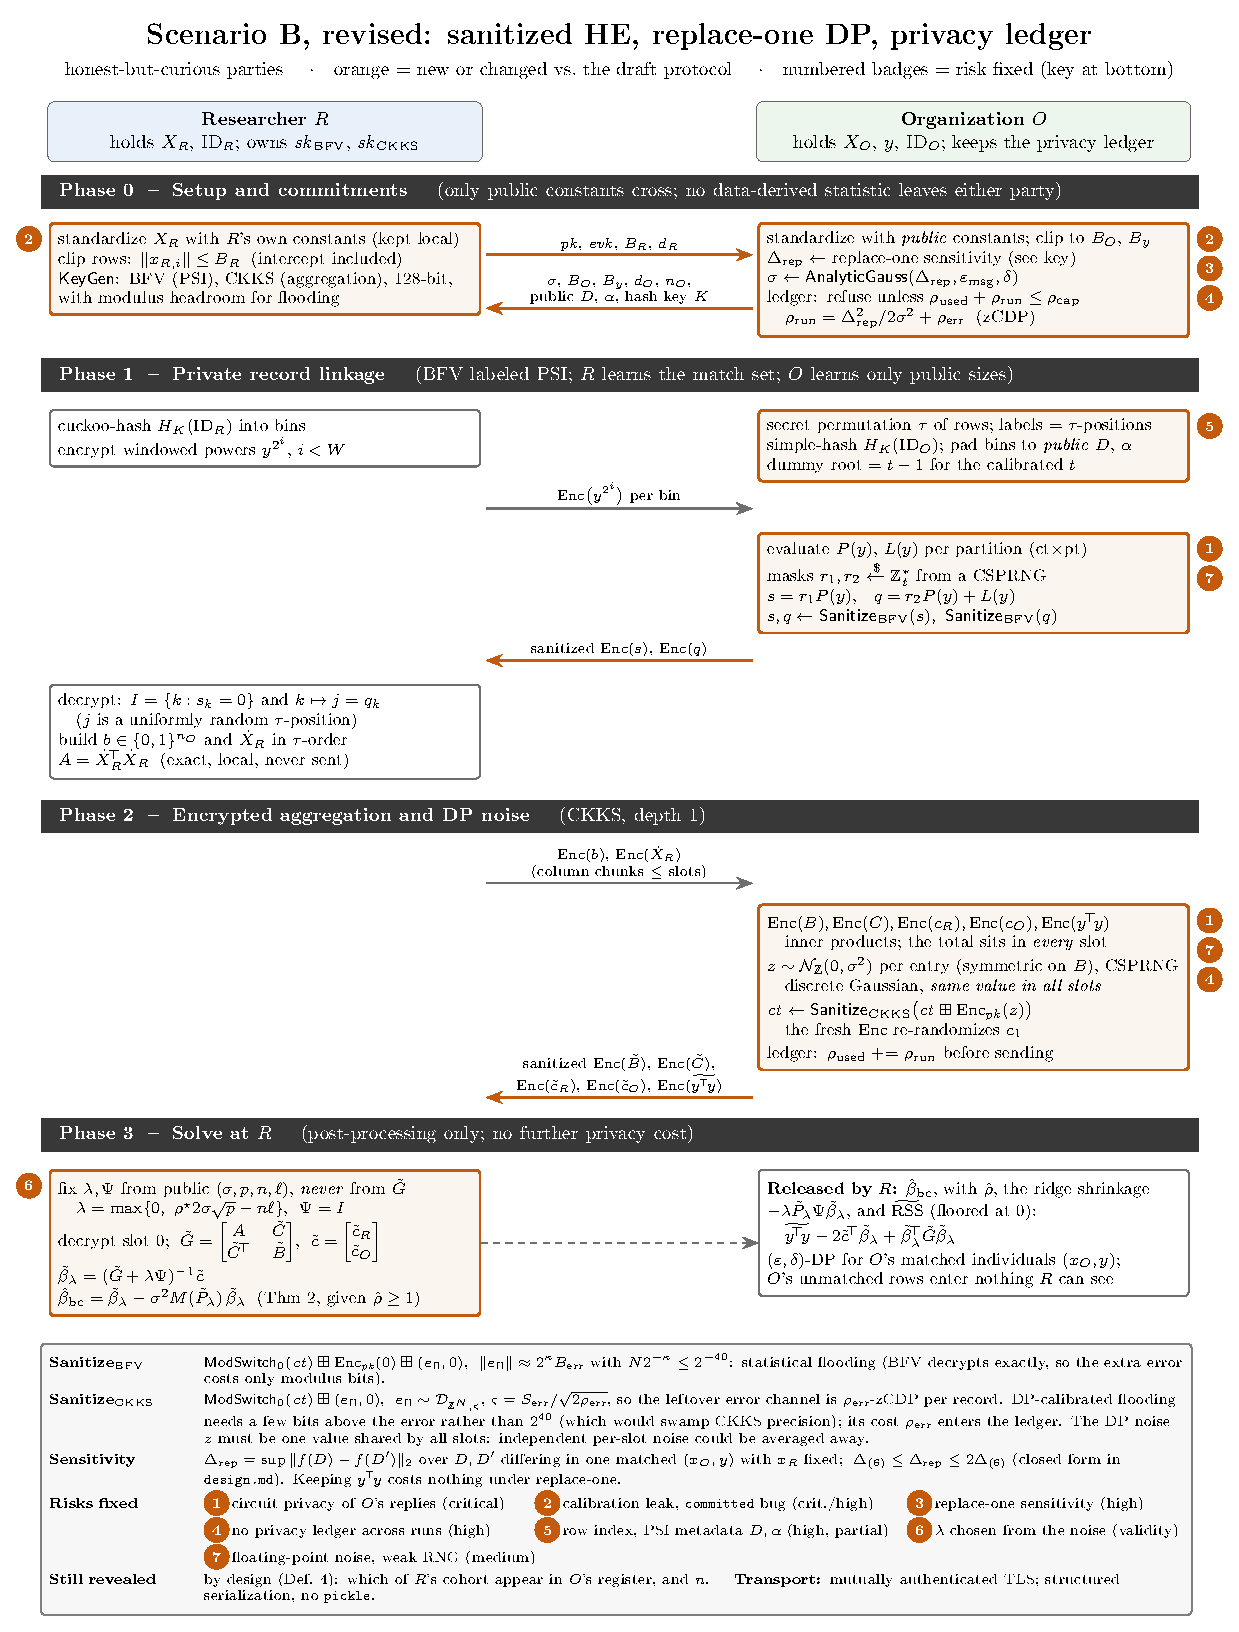
\includegraphics[width=\textwidth,height=0.85\textheight,keepaspectratio]{figures/protocol_v2.pdf}
  \caption{Message flow of Protocol~\ref{prot:scenB}. Orange marks steps that are new or changed relative to the earlier specification; numbered badges refer to the risks listed in the figure's key.}
  \label{fig:protocol}
\end{figure}

\subsection{Protocol}

\begin{protocol}[Revised Scenario-B protocol]
\label{prot:scenB}
\hfill

\smallskip
\textbf{Phase 0 --- Setup and commitments (Alg.~\ref{alg:setup}).}
$\Party{R}$ standardizes $\bXR$ with its own constants, which never leave $\Party{R}$, clips rows to the committed bound $B_{R}$, and generates a BFV key pair for linkage and a CKKS key pair for aggregation, both at 128-bit security with modulus headroom for flooding. $\Party{O}$ standardizes $(\bXO, \by)$ with \emph{public} constants and clips to $B_{O}$ and $B_{y}$, computes the replace-one sensitivity $\Delta$ (Proposition~\ref{prop:sens}) and $\sigma$, and refuses the run if its privacy ledger would exceed the cap. Only public constants cross in either direction.

\smallskip
\textbf{Phase 1 --- Private record linkage (Alg.~\ref{alg:link}, Appendix~\ref{app:psi}).}
$\Party{O}$ applies a secret permutation $\tau$ to its rows. The parties run labeled PSI, in which $\Party{R}$ sends encrypted windowed powers of its keyed-hashed identifiers and $\Party{O}$ returns masked, sanitized evaluations of its membership and label polynomials, padded to public degrees. $\Party{R}$ obtains $I$ and $\pi$, the labels being uniformly random $\tau$-positions; $\Party{O}$ learns only public sizes. $\Party{R}$ builds $\bb$ and $\dXR$ and computes
\[
  \bA = \dXR^{\top}\dXR = \sum_{k \in I} \mathbf{x}_{R,k}\mathbf{x}_{R,k}^{\top} \in \R^{d_{R} \times d_{R}}
\]
locally; $\bA$ is retained through to the solve and never transmitted.

\smallskip
\textbf{Phase 2 --- Encrypted aggregation and DP noise (Alg.~\ref{alg:aggregate}).}
$\Party{R}$ sends $\Enc{\bb}$ and $\Enc{\dXR}$ in column chunks of at most the slot count. Using plaintext $\bXO$ and $\by$, all at multiplicative depth one, $\Party{O}$ computes
\begin{align}
  \Enc{B_{jk}} &= \sum_{i} \Enc{b_{i}}\,X_{O,ij}X_{O,ik}, &
  \Enc{C_{jk}} &= \sum_{i} \Enc{\dot{X}_{R,ij}}\,X_{O,ik}, \label{eq:BC}\\
  \Enc{c_{O,k}} &= \sum_{i} \Enc{b_{i}}\,X_{O,ik}\,y_{i}, &
  \Enc{c_{R,j}} &= \sum_{i} \Enc{\dot{X}_{R,ij}}\,y_{i}, \label{eq:cOcR}
\end{align}
and $\Enc{\by^{\top}\by} = \sum_{i}\Enc{b_{i}}\,y_{i}^{2}$, each inner product leaving the total in every slot. ($\bC$ needs no $\bb$, since $\dXR$ is already zero off the matched set; $\bcR$ is the central cross-term, in which $\Party{O}$ multiplies $\Party{R}$'s encrypted features by its own plaintext outcome.) For every released entry $\Party{O}$ draws discrete-Gaussian noise $z \sim \mathcal{N}_{\Z/\gamma}(0,\sigma^{2})$ (symmetric on $\bB$), adds a \emph{fresh encryption} of $z$ carried identically in every slot, and sanitizes the result (Section~\ref{sec:circuit}). $\Party{O}$ records the run in its ledger before sending.

\smallskip
\textbf{Phase 3 --- Solve at $\Party{R}$ (Alg.~\ref{alg:solve}).}
$\Party{R}$ fixes the ridge $(\lambda, \Psi)$ from public inputs \emph{before} decrypting (Section~\ref{sec:bias:lambda}), decrypts slot~0 of each ciphertext, splices in its exact local $\bA$,
\[
  \tilde{\bG} = \begin{bmatrix} \bA & \tilde{\bC} \\ \tilde{\bC}^{\top} & \tilde{\bB} \end{bmatrix}, \qquad
  \tilde{\bc} = \begin{bmatrix} \tilde{\bc}_{R} \\ \tilde{\bc}_{O} \end{bmatrix},
\]
solves $\tilde{\bbeta}_{\lambda} = (\tilde{\bG} + \lambda\Psi)^{-1}\tilde{\bc}$, and applies the zero-budget bias correction of Section~\ref{sec:bias:correction}. It releases $\hat{\bbeta}_{\mathrm{bc}}$ together with the validity statistic $\hat{\rho}$, the deterministic ridge shrinkage, and $\widetilde{\mathrm{RSS}}$.
\end{protocol}

\subsection{Direction-of-data ledger}

\begin{table}[ht]
\centering
\renewcommand{\arraystretch}{1.25}
\begin{tabular}{@{}l>{\raggedright\arraybackslash}p{10.6cm}@{}}
\toprule
$\Party{R} \to \Party{O}$ & $\pk_{B}$, $\pk_{C}$, evaluation keys; $B_{R}$, $d_{R}$, $n_{R}$; BFV encryptions of windowed powers of hashed identifiers; $\Enc{\bb}$, $\Enc{\dXR}$ \\
$\Party{O} \to \Party{R}$ & $\sigma$, $B_{O}$, $B_{y}$, $d_{O}$, $n_{O}$, public $(D,\alpha)$, hash key $K$, public standardization constants; sanitized PSI replies; sanitized $\Enc{\tilde{\bB}}$, $\Enc{\tilde{\bC}}$, $\Enc{\tilde{\bc}_{R}}$, $\Enc{\tilde{\bc}_{O}}$, $\Enc{\widetilde{\by^{\top}\by}}$ \\
never transmitted & $\bA$ (local to $\Party{R}$); $\by$ (local to $\Party{O}$); $\sk_{B}$, $\sk_{C}$; raw $\bXR$, $\bXO$; $\tau$; the noise draws; any statistic computed from either party's data other than the released noisy aggregates \\
\bottomrule
\end{tabular}
\caption{What crosses between the parties. All messages travel over a mutually authenticated TLS channel with structured (non-executable) serialization.}
\label{tab:ledger}
\end{table}

Under Definition~\ref{def:adj}, $\bA$ is a deterministic function of $(I, \bXR)$, both known to $\Party{R}$; it carries no incremental information about $\Party{O}$ and correctly receives no noise.

\begin{remark}[Corrections relative to the earlier specification]
\label{rem:corrections}
\begin{enumerate}[noitemsep, label=(\roman*)]
  \item $\Party{R}$ no longer uploads $\Enc{\bA}$. $\Party{O}$ never consumes $\bA$; the final solve occurs at $\Party{R}$, which forms $\bA$ from its own records the moment linkage completes. Keeping $\bA$ local is lossless, and it is what makes the top-left block of the Gram noise vanish (Section~\ref{sec:bias}).
  \item The DP noise is added by a fresh encryption followed by sanitization, not by a plaintext-scalar addition (Section~\ref{sec:circuit}).
  \item The noise is calibrated to the replace-one sensitivity that Definition~\ref{def:adj} requires, not to the add/remove bound (Section~\ref{sec:dp:sens}).
  \item Calibration is split between the parties: no statistic derived from either party's data (quantiles, clip rates, sample means or standard deviations) is exchanged.
  \item $\Party{O}$ keeps a privacy ledger, so that re-runs and retraining compose under an explicit cap.
  \item The ridge is fixed from public inputs rather than chosen from the noisy Gram (Section~\ref{sec:bias:lambda}).
  \item The linkage uses labeled PSI with data-independent labels and metadata (Appendix~\ref{app:psi}).
\end{enumerate}
\end{remark}

% ==============================================================
% Pseudocode for the revised Scenario-B protocol.
% Requires: algorithm, algpseudocode, and the macros of main.tex.
% ==============================================================

\algnewcommand{\AtParty}[1]{\Statex \hspace*{-\algorithmicindent}\textit{At $\Party{#1}$:}}
\algnewcommand{\SendTo}[2]{\State \textbf{send} #1 \textbf{to} $\Party{#2}$}
\algrenewcommand\algorithmicrequire{\textbf{Input:}}
\algrenewcommand\algorithmicensure{\textbf{Output:}}

% --------------------------------------------------------------
\begin{algorithm}[p]
\caption{\textsc{Setup}: commitments and calibration (Phase~0)}
\label{alg:setup}
\small
\begin{algorithmic}[1]
\Require $\Party{R}$: $\bXR$, $\mathit{ID}_{R}$. \;
  $\Party{O}$: $\bXO$, $\by$, $\mathit{ID}_{O}$, public standardization constants
  $(\boldsymbol{\mu}_{O}, \mathbf{s}_{O}, \mu_{y}, s_{y})$, privacy ledger $\mathcal{L}$,
  cap $\rho_{\mathrm{cap}}$. \;
  Public: $(\varepsilon_{\mathrm{msg}}, \delta)$, $\rho_{\mathrm{err}}$, HE parameters,
  PSI parameters $(N_{\mathrm{bins}}, h, d_{\mathrm{cap}}, W)$, flooding parameter $\kappa$.
\Ensure Public parameter set $\mathcal{P}$; $\Party{R}$ holds $(\sk_{B}, \sk_{C})$.
\AtParty{R}
\State Standardize $\bXR$ with $\Party{R}$'s own constants, which never leave $\Party{R}$;
  append the intercept column if one is used
\State $\mathbf{x}_{R,k} \gets \mathbf{x}_{R,k}\cdot\min\{1,\, B_{R}/\|\mathbf{x}_{R,k}\|_{2}\}$
  for all $k \in [n_{R}]$ \Comment{enforce the committed bound}
\State $(\pk_{B}, \sk_{B}, \mathit{evk}_{B}) \gets \mathsf{BFV.KeyGen}(N_{B}, t, q_{B})$;\;
  $(\pk_{C}, \sk_{C}, \mathit{evk}_{C}) \gets \mathsf{CKKS.KeyGen}(N_{C}, \Delta_{C}, q_{C})$
  \Comment{128-bit; $q$ includes flooding headroom}
\SendTo{$(\pk_{B}, \mathit{evk}_{B}, \pk_{C}, \mathit{evk}_{C}, B_{R}, d_{R}, n_{R})$}{O}
\AtParty{O}
\State Standardize $(\bXO, \by)$ with the public constants; clip
  $\|\mathbf{x}_{O,i}\|_{2} \le B_{O}$ and $|y_{i}| \le B_{y}$ for all $i \in [n_{O}]$
\State $\Delta \gets \textsc{DeltaRep}(B_{R}, B_{O}, B_{y})$ \Comment{replace-one sensitivity, Alg.~\ref{alg:sub}}
\State $\sigma \gets \textsc{AnalyticGauss}(\Delta, \varepsilon_{\mathrm{msg}}, \delta)$;\quad
  $\rho_{\mathrm{run}} \gets \Delta^{2}/(2\sigma^{2}) + \rho_{\mathrm{err}}$
\If{$\mathcal{L}[\Party{R}, \text{dataset}] + \rho_{\mathrm{run}} > \rho_{\mathrm{cap}}$}
  \State \textbf{abort} \Comment{budget exhausted}
\EndIf
\State $K \xleftarrow{\$} \{0,1\}^{256}$;\;
  $(D, \alpha) \gets$ public degree and partition count computed from $(n_{O}, h, N_{\mathrm{bins}}, d_{\mathrm{cap}})$
\SendTo{$\mathcal{P} = (\sigma, B_{O}, B_{y}, d_{O}, n_{O}, D, \alpha, K,
  \boldsymbol{\mu}_{O}, \mathbf{s}_{O}, \mu_{y}, s_{y})$}{R}
\end{algorithmic}
\end{algorithm}

% --------------------------------------------------------------
\begin{algorithm}[p]
\caption{\textsc{Link}: labeled PSI with record alignment (Phase~1)}
\label{alg:link}
\small
\begin{algorithmic}[1]
\Require $\Party{R}$: $\mathit{ID}_{R}$, $\bXR$, $\sk_{B}$. \;
  $\Party{O}$: $\mathit{ID}_{O}$, rows $(\mathbf{x}_{O,i}, y_{i})_{i \in [n_{O}]}$. \;
  Public: $K$, $t$, $N_{\mathrm{bins}}$, hash functions $\beta_{1}, \dots, \beta_{h}$, $D$, $\alpha$, $W$.
\Ensure $\Party{R}$: $I$, $\pi$, $\bb$, $\dXR$, $\bA$. \; $\Party{O}$: nothing.
\AtParty{O} \Comment{offline preprocessing}
\State $\tau \xleftarrow{\$} \mathrm{Sym}(n_{O})$; re-index the rows of $(\mathit{ID}_{O}, \bXO, \by)$ by $\tau$
  \Comment{uniform labels}
\State $v_{j} \gets H_{K}(\mathit{ID}_{O,j}) \bmod (t-1)$ for $j \in [n_{O}]$
  \Comment{never equals the dummy root $t-1$}
\State Insert $(v_{j}, j)$ into bins $\beta_{1}(v_{j}), \dots, \beta_{h}(v_{j})$ \Comment{simple hashing}
\If{a bin holds more than $\alpha D$ items, or two items in one bin share a value $v$}
  \State \textbf{abort} \Comment{probability $\le \delta_{\mathrm{psi}}$}
\EndIf
\For{each bin $\beta \in [N_{\mathrm{bins}}]$ and partition $a \in [\alpha]$}
  \State $S_{\beta,a} \gets$ the $a$-th block of at most $D$ items in bin $\beta$
  \State $P_{\beta,a}(X) \gets \prod_{(v,j) \in S_{\beta,a}} (X - v) \cdot (X - (t-1))^{D - |S_{\beta,a}|}$
    \Comment{padded to the public degree $D$}
  \State $L_{\beta,a} \gets$ the interpolant of degree $< D$ with $L_{\beta,a}(v) = j$ for all $(v,j) \in S_{\beta,a}$
\EndFor
\AtParty{R}
\State $u_{k} \gets H_{K}(\mathit{ID}_{R,k}) \bmod (t-1)$; cuckoo-insert every $u_{k}$ into $N_{\mathrm{bins}}$ bins
  using $\beta_{1}, \dots, \beta_{h}$; let $T[\beta] = k$ for occupied bins \Comment{batches if $n_{R}$ exceeds capacity}
\State $w_{\beta} \gets u_{T[\beta]}$ for occupied bins, $w_{\beta} \gets 0$ otherwise
\SendTo{$\mathsf{BFV.Enc}_{\pk_{B}}\bigl(\mathbf{w}^{\odot 2^{i}}\bigr)$ for $i = 0, \dots, W-1$}{O}
\AtParty{O}
\State $\mathit{ct}_{d} \gets \mathsf{Enc}(\mathbf{w}^{\odot d})$ for $d = 1, \dots, D$, as products of window ciphertexts
\For{$a = 1, \dots, \alpha$}
  \State $\mathit{ct}_{P} \gets \mathbf{p}_{a,0} \boxplus \bigboxplus_{d=1}^{D} \mathbf{p}_{a,d} \odot \mathit{ct}_{d}$;\quad
    $\mathit{ct}_{L} \gets \boldsymbol{\ell}_{a,0} \boxplus \bigboxplus_{d=1}^{D-1} \boldsymbol{\ell}_{a,d} \odot \mathit{ct}_{d}$
    \Comment{also valid for $D=1$}
  \State $\mathbf{r}_{1}, \mathbf{r}_{2} \xleftarrow{\$} (\mathbb{Z}_{t}^{\ast})^{N_{\mathrm{bins}}}$ from a CSPRNG
  \State $\mathit{ct}_{s} \gets \textsc{SanitizeBFV}(\mathbf{r}_{1} \odot \mathit{ct}_{P})$;\quad
    $\mathit{ct}_{q} \gets \textsc{SanitizeBFV}(\mathbf{r}_{2} \odot \mathit{ct}_{P} \boxplus \mathit{ct}_{L})$
  \SendTo{$(\mathit{ct}_{s}, \mathit{ct}_{q})$}{R}
\EndFor
\AtParty{R}
\For{each occupied bin $\beta$ with $k = T[\beta]$, and each $a \in [\alpha]$}
  \State $s \gets \mathsf{Dec}_{\sk_{B}}(\mathit{ct}_{s}^{(a)})_{\beta}$;\; $q \gets \mathsf{Dec}_{\sk_{B}}(\mathit{ct}_{q}^{(a)})_{\beta}$
  \If{$s = 0$ \textbf{and} $0 \le q < n_{O}$} \State $\pi(k) \gets q$ \EndIf
\EndFor
\State $I \gets \mathrm{dom}(\pi)$;\; $\bb \gets \mathbf{0}_{n_{O}}$;\; $\dXR \gets \mathbf{0}_{n_{O} \times d_{R}}$
\State \textbf{for} $k \in I$: $b_{\pi(k)} \gets 1$ and $\dXR[\pi(k), :] \gets \mathbf{x}_{R,k}^{\top}$
\State $\bA \gets \dXR^{\top}\dXR$ \Comment{exact; never transmitted}
\end{algorithmic}
\end{algorithm}

% --------------------------------------------------------------
\begin{algorithm}[p]
\caption{\textsc{Aggregate}: encrypted sufficient statistics with DP noise (Phase~2)}
\label{alg:aggregate}
\small
\begin{algorithmic}[1]
\Require $\Party{R}$: $\bb$, $\dXR$, $\pk_{C}$. \;
  $\Party{O}$: $\bXO$, $\by$ in $\tau$-order, $\sigma$, $\rho_{\mathrm{run}}$, ledger $\mathcal{L}$. \;
  Public: slot count $S$.
\Ensure $\Party{R}$ receives sanitized encryptions of
  $\tilde{\bB}$, $\tilde{\bC}$, $\tilde{\mathbf{c}}_{R}$, $\tilde{\mathbf{c}}_{O}$, $\widetilde{\by^{\top}\by}$.
\AtParty{R}
\State Partition $[n_{O}]$ into chunks $\mathcal{C}_{1}, \dots, \mathcal{C}_{m}$ of at most $S$ positions
\SendTo{$\mathsf{CKKS.Enc}(\bb_{\mathcal{C}_{c}})$ and $\mathsf{CKKS.Enc}(\dXR[\mathcal{C}_{c}, j])$
  for all $c \in [m]$, $j \in [d_{R}]$}{O}
\AtParty{O}
\State $\mathcal{E} \gets \{(\bb, \mathbf{x}_{O,\cdot j} \odot \mathbf{x}_{O,\cdot k}) : j \le k\}
  \cup \{(\dXR[:,j], \mathbf{x}_{O,\cdot k})\}
  \cup \{(\dXR[:,j], \by)\}
  \cup \{(\bb, \mathbf{x}_{O,\cdot k} \odot \by)\}
  \cup \{(\bb, \by \odot \by)\}$
\Statex \hspace*{\algorithmicindent}\Comment{(encrypted, plaintext) pairs giving $B_{jk}$, $C_{jk}$, $c_{R,j}$, $c_{O,k}$, $\by^{\top}\by$}
\For{each $(\mathbf{u}, \mathbf{w}) \in \mathcal{E}$}
  \State $\mathit{ct} \gets \bigboxplus_{c=1}^{m} \mathsf{EvalSum}\bigl(\mathsf{Enc}(\mathbf{u}_{\mathcal{C}_{c}}) \odot \mathbf{w}_{\mathcal{C}_{c}}\bigr)$
    \Comment{depth 1; the total occupies every slot}
  \State $z \gets \mathcal{N}_{\mathbb{Z}/\gamma}(0, \sigma^{2})$ from a CSPRNG
    \Comment{discrete Gaussian at resolution $1/\gamma$; one draw per released entry}
  \State $\mathit{ct} \gets \textsc{SanitizeCKKS}\bigl(\mathit{ct} \boxplus \mathsf{CKKS.Enc}_{\pk_{C}}(z \cdot \mathbf{1})\bigr)$
    \Comment{same $z$ in every slot; fresh $c_{1}$}
\EndFor
\State $\mathcal{L}[\Party{R}, \text{dataset}] \gets \mathcal{L}[\Party{R}, \text{dataset}] + \rho_{\mathrm{run}}$
  \Comment{recorded before release}
\SendTo{all sanitized ciphertexts}{R}
\end{algorithmic}
\end{algorithm}

% --------------------------------------------------------------
\begin{algorithm}[p]
\caption{\textsc{Solve}: assembly, fixed ridge and bias correction at $\Party{R}$ (Phase~3)}
\label{alg:solve}
\small
\begin{algorithmic}[1]
\Require $\Party{R}$: $\bA$, $\sk_{C}$, the ciphertexts of Alg.~\ref{alg:aggregate}. \;
  Public: $\sigma$, $p = d_{R} + d_{O}$, $n = |I|$, validity target $\rho^{\star}$, committed eigenvalue floor $\ell \ge 0$.
\Ensure $\hat{\bbeta}_{\mathrm{bc}}$, the validity statistic $\hat{\rho}$, the ridge shrinkage $\mathbf{s}_{\lambda}$, and $\widetilde{\mathrm{RSS}}$.
\State $\lambda \gets \max\{0,\; 2\rho^{\star}\sigma\sqrt{p} - n\ell\}$;\quad $\Psi \gets \mathbf{I}_{p}$
  \Comment{fixed before decryption, never from $\tilde{\bG}$}
\State Decrypt slot 0 of every ciphertext; set $\tilde{B}_{kj} \gets \tilde{B}_{jk}$ for $j < k$
\State $\tilde{\bG} \gets \begin{bmatrix} \bA & \tilde{\bC} \\ \tilde{\bC}^{\top} & \tilde{\bB} \end{bmatrix}$;\quad
  $\tilde{\mathbf{c}} \gets \begin{bmatrix} \tilde{\mathbf{c}}_{R} \\ \tilde{\mathbf{c}}_{O} \end{bmatrix}$
\State $\hat{\rho} \gets \lambda_{\min}(\tilde{\bG} + \lambda\Psi) / (2\sigma\sqrt{p})$
\If{$\hat{\rho} < 1$}
  \State report that the validity check failed and withhold $\hat{\bbeta}$ \Comment{post-processing; no privacy cost}
\EndIf
\State $\tilde{\bP} \gets (\tilde{\bG} + \lambda\Psi)^{-1}$;\quad $\tilde{\bbeta} \gets \tilde{\bP}\tilde{\mathbf{c}}$
\State $\hat{\bbeta}_{\mathrm{bc}} \gets \tilde{\bbeta} - \sigma^{2}\,\textsc{BiasOp}(\tilde{\bP}, d_{R})\,\tilde{\bbeta}$ \Comment{Theorem~\ref{thm:ridge}}
\State $\mathbf{s}_{\lambda} \gets -\lambda\tilde{\bP}\Psi\tilde{\bbeta}$;\quad
  $\widetilde{\mathrm{RSS}} \gets \max\bigl\{0,\; \widetilde{\by^{\top}\by} - 2\tilde{\mathbf{c}}^{\top}\tilde{\bbeta} + \tilde{\bbeta}^{\top}\tilde{\bG}\tilde{\bbeta}\bigr\}$
\State \Return $\hat{\bbeta}_{\mathrm{bc}}, \hat{\rho}, \mathbf{s}_{\lambda}, \widetilde{\mathrm{RSS}}$,
  back-transformed with $\Party{R}$'s constants and $\Party{O}$'s public constants
\end{algorithmic}
\end{algorithm}

% --------------------------------------------------------------
\begin{algorithm}[p]
\caption{Subroutines}
\label{alg:sub}
\small
\begin{algorithmic}[1]
\Function{SanitizeBFV}{$\mathit{ct}$} \Comment{statistical flooding; BFV decryption stays exact}
  \State $\mathit{ct} \gets \mathsf{ModSwitch}_{0}(\mathit{ct})$
  \State $\mathbf{e} \gets \mathcal{D}_{\mathbb{Z}^{N_{B}},\, 2^{\kappa} B_{\mathrm{err}}}$
    \Comment{$B_{\mathrm{err}}$: bound on the error of $\mathit{ct}$ at level 0}
  \State \Return $\mathit{ct} \boxplus \mathsf{BFV.Enc}_{\pk_{B}}(\mathbf{0}) \boxplus (\mathbf{e}, 0)$
\EndFunction
\Statex
\Function{SanitizeCKKS}{$\mathit{ct}$} \Comment{DP-calibrated flooding of the error channel}
  \State $\mathit{ct} \gets \mathsf{ModSwitch}_{0}(\mathit{ct})$
  \State $\varsigma \gets S_{\mathrm{err}} / \sqrt{2\rho_{\mathrm{err}}}$;\quad
    $\mathbf{e} \gets \mathcal{D}_{\mathbb{Z}^{N_{C}},\, \varsigma}$
    \Comment{Lemma~\ref{lem:flood}}
  \State \Return $\mathit{ct} \boxplus (\mathbf{e}, 0)$
\EndFunction
\Statex
\Function{DeltaRep}{$B_{R}, B_{O}, B_{y}$} \Comment{Proposition~\ref{prop:sens}}
  \State $R \gets B_{R}^{2}$,\; $O \gets B_{O}^{2}$,\; $Y \gets B_{y}^{2}$
  \If{$|R - Y| \le 2O$} \State \Return $\bigl(\tfrac12(2O + R + Y)^{2} + 2RY\bigr)^{1/2}$
  \ElsIf{$R - Y \ge 2O$} \State \Return $\bigl(4R(O + Y)\bigr)^{1/2}$
  \Else \State \Return $\bigl(\max_{t \in [-B_{y}, B_{y}]} F(c^{\ast}(t), t)\bigr)^{1/2}$ \Comment{$F$, $c^{\ast}$ as in \eqref{eq:sens_F}}
  \EndIf
\EndFunction
\Statex
\Function{AnalyticGauss}{$\Delta, \varepsilon, \delta$} \Comment{Balle--Wang}
  \State \Return the smallest $\sigma$ with
    $\Phi\bigl(\tfrac{\Delta}{2\sigma} - \tfrac{\varepsilon\sigma}{\Delta}\bigr)
     - e^{\varepsilon}\,\Phi\bigl(-\tfrac{\Delta}{2\sigma} - \tfrac{\varepsilon\sigma}{\Delta}\bigr) \le \delta$
    \Comment{bisection}
\EndFunction
\Statex
\Function{BiasOp}{$\mathbf{P}, d_{R}$} \Comment{bracket of Theorem~\ref{thm:bias}}
  \State $\Pi_{R} \gets \mathrm{diag}(\mathbf{1}_{d_{R}}, \mathbf{0}_{d_{O}})$;\; $\Pi_{O} \gets \mathbf{I}_{p} - \Pi_{R}$
  \State \Return $\bigl(\mathbf{P}^{2} + \mathrm{tr}(\mathbf{P})\mathbf{P} - \mathbf{P}\,\mathrm{diag}(\mathbf{P})\bigr)\Pi_{O}
    + \bigl(\mathbf{P}\Pi_{O}\mathbf{P} + \mathrm{tr}(\Pi_{O}\mathbf{P})\mathbf{P}\bigr)\Pi_{R}$
\EndFunction
\end{algorithmic}
\end{algorithm}


% ==============================================================
\section{Output Privacy: DP Noise on Encrypted Aggregates}
\label{sec:dp}
% ==============================================================

\subsection{The noise injection mechanism}
\label{sec:dp:mech}

For every released entry $s$ of the stacked statistic
\begin{equation}
  \mathbf{f}(D) = \bigl(\mathrm{triu}(\bB),\; \bC,\; \bcR,\; \bcO,\; \by^{\top}\by\bigr),
  \label{eq:release}
\end{equation}
$\Party{O}$ draws $z_{s} \sim \mathcal{N}_{\Z/\gamma}(0, \sigma^{2})$ independently (a discrete Gaussian on the grid $\gamma^{-1}\Z$ at the CKKS resolution~\cite{canonne2020discrete}), mirrors the draws for $\bB$ across the diagonal, and sets
\begin{equation}
  \mathit{ct}_{s} \;\gets\; \textsc{SanitizeCKKS}\bigl(\Enc{s} \boxplus \mathsf{Enc}_{\pk_{C}}(z_{s}\cdot\mathbf{1})\bigr).
  \label{eq:noise_inject}
\end{equation}
$\Party{O}$ retains $z_{s}$ and never discloses it; $\Party{R}$ decrypts $\tilde{s} = s + z_{s}$ (up to a CKKS perturbation far below $\sigma$) and cannot decompose it. Two details matter:
\begin{itemize}[noitemsep]
  \item \emph{The same $z_{s}$ in every slot.} The inner products of~\eqref{eq:BC}--\eqref{eq:cOcR} leave the total in all $N_{C}/2$ slots. Independent noise per slot would let $\Party{R}$ average the copies and remove the noise; the constant vector $z_{s}\mathbf{1}$ gives every copy the same noise.
  \item \emph{A fresh encryption, then sanitization.} A plaintext-scalar addition would not re-randomize the ciphertext; Section~\ref{sec:circuit} shows this is fatal.
\end{itemize}
Because $\sigma$ is a public constant chosen by $\Party{O}$, the privacy budget stays under $\Party{O}$'s control, and every function of the released statistics computed by $\Party{R}$ from its own data inherits the guarantee by post-processing.

\subsection{Sensitivity under replace-one adjacency}
\label{sec:dp:sens}

A subtlety arises for $B_{R}$: because $\bXR$ is encrypted, $\Party{O}$ cannot compute $\|\mathbf{x}_{R,k}\|_{2}$ directly. $\Party{R}$ must commit to $B_{R}$ during setup, before any data is exchanged, and enforce it by clipping; this allows $\Party{O}$ to calibrate the noise without seeing the data. If $\Party{R}$ appends an intercept column, the committed bound is $\sqrt{1 + B_{R,\mathrm{rows}}^{2}}$.

Replacing one matched individual's $(\mathbf{x}, y)$ by $(\mathbf{x}', y')$ with $\mathbf{x}_{R}$ fixed changes the released vector by
\[
  \bigl(\mathrm{triu}(\mathbf{x}\mathbf{x}^{\top} - \mathbf{x}'\mathbf{x}'^{\top}),\;
  \mathbf{x}_{R}(\mathbf{x} - \mathbf{x}')^{\top},\;
  \mathbf{x}_{R}(y - y'),\;
  \mathbf{x}y - \mathbf{x}'y',\;
  y^{2} - y'^{2}\bigr).
\]
Let $\Delta = \sup \|\mathbf{f}(D) - \mathbf{f}(D')\|_{2}$ over adjacent $D, D'$, and let
\begin{equation}
  \Delta_{\mathrm{add}}^{2} = (B_{O}^{2} + B_{R}^{2})(B_{O}^{2} + B_{y}^{2}) + B_{y}^{4}
  \label{eq:sens_add}
\end{equation}
be the bound obtained when one record is added or removed. The earlier specification used~\eqref{eq:sens_add}, which does not match Definition~\ref{def:adj}.

\begin{proposition}[Replace-one sensitivity]
\label{prop:sens}
$\Delta_{\mathrm{add}} \le \Delta \le 2\Delta_{\mathrm{add}}$. Moreover, with $R = B_{R}^{2}$, $O = B_{O}^{2}$, $Y = B_{y}^{2}$,
\begin{equation}
  \Delta^{2} =
  \begin{cases}
    \tfrac12(2O + R + Y)^{2} + 2RY & \text{if } |R - Y| \le 2O,\\[2pt]
    4R(O + Y) & \text{if } R - Y \ge 2O,\\[2pt]
    \max_{t \in [-B_{y}, B_{y}]} F\bigl(c^{\ast}(t), t\bigr) & \text{if } Y - R > 2O,
  \end{cases}
  \label{eq:sens_closed}
\end{equation}
where
\begin{equation}
\begin{aligned}
  F(c,t) &= 2O^{2}(1 - c^{2}) + 2RO(1 - c) + R(B_{y} - t)^{2}\\
         &\quad + O(Y + t^{2}) - 2OcB_{y}t + (Y - t^{2})^{2},\\
  c^{\ast}(t) &= \min\bigl\{1, \max\{-1, -(R + B_{y}t)/(2O)\}\bigr\}.
\end{aligned}
\label{eq:sens_F}
\end{equation}
\end{proposition}

\begin{proof}[Proof sketch]
The lower bound follows by replacing $(\mathbf{x}, y)$ with $(\mathbf{0}, 0)$, which reproduces the add/remove change. For the upper bound, write $\mathbf{f}(D) - \mathbf{f}(D') = [\mathbf{f}(D) - \mathbf{f}(D^{0})] + [\mathbf{f}(D^{0}) - \mathbf{f}(D')]$, where $D^{0}$ has the individual's $\Party{O}$-side data set to zero, and apply the triangle inequality. For~\eqref{eq:sens_closed}, the objective is increasing in $\|\mathbf{x}_{R}\|$, so $\|\mathbf{x}_{R}\| = B_{R}$; at the optimum $\|\mathbf{x}\| = \|\mathbf{x}'\| = B_{O}$ and $|y| = B_{y}$, and the remaining dependence is on $c = \cos\angle(\mathbf{x}, \mathbf{x}')$ and $t = y'$. Maximizing the concave quadratic in $c$ gives $c^{\ast}(t)$, and the three cases correspond to where the maximizer in $t$ lies. The closed form agrees with brute-force maximization to within $5\times10^{-9}$ relative on fifteen bound settings covering all three regimes (\texttt{reports/checks/replace\_one\_closed\_form\_check.py}). In the third regime the one-dimensional maximum must be computed with local refinement or rounded up, since $\sigma$ must never be calibrated to an underestimate.
\end{proof}

\begin{remark}[Magnitude, and $\by^{\top}\by$ is free]
For $B_{R} = B_{O} = B_{y}$ the ratio $\Delta/\Delta_{\mathrm{add}}$ is $\sqrt{2}$; it approaches $2$ when $B_{R}$ dominates (many $\Party{R}$ features, or the intercept) and $1$ when $B_{y}$ dominates. For $B_{R} = B_{O} = \sqrt{5}$, $B_{y} = 5$ it is $31.6/30.4$. Releasing $\by^{\top}\by$ costs nothing under replace-one: the worst case replaces $(\mathbf{x}, y)$ with $(-\mathbf{x}, -y)$, which leaves $y^{2}$ unchanged, and $\Delta$ is numerically identical with or without $\by^{\top}\by$ in all settings we checked.
\end{remark}

The upper triangle of $\bB$, rather than the full matrix, is what is released and noised; using the full Frobenius norm of $\Delta\bB$ would be conservative.

\subsection{Calibration, composition and the ledger}

$\Party{O}$ calibrates $\sigma$ with the analytic Gaussian mechanism of Balle and Wang~\cite{balle2018improving}: the smallest $\sigma$ with
\[
  \Phi\Bigl(\tfrac{\Delta}{2\sigma} - \tfrac{\varepsilon\sigma}{\Delta}\Bigr)
  - e^{\varepsilon}\,\Phi\Bigl(-\tfrac{\Delta}{2\sigma} - \tfrac{\varepsilon\sigma}{\Delta}\Bigr) \le \delta ,
\]
evaluating the left tail with $\tfrac12\mathrm{erfc}$ to avoid cancellation. Whatever rule chooses $\sigma$, the (discrete) Gaussian mechanism with $\ell_{2}$-sensitivity $\Delta$ is $\rho$-zCDP with $\rho = \Delta^{2}/(2\sigma^{2})$~\cite{bun2016concentrated,canonne2020discrete}; zCDP composes additively and converts to $(\varepsilon,\delta)$-DP with $\varepsilon = \rho + 2\sqrt{\rho\ln(1/\delta)}$.

$\Party{O}$ therefore keeps a ledger per (dataset, researcher). A run costs
\begin{equation}
  \rho_{\mathrm{run}} = \frac{\Delta^{2}}{2\sigma^{2}} + \rho_{\mathrm{err}},
  \label{eq:rho_run}
\end{equation}
where $\rho_{\mathrm{err}}$ is the cost of the ciphertext-error channel (Lemma~\ref{lem:flood}); $\Party{O}$ refuses a run if the cumulative spend would exceed its cap $\rho_{\mathrm{cap}}$, and records the spend before releasing. Retraining, re-runs, and the per-query noise of split inference (Section~\ref{sec:inf:split}) are all charged to the same ledger.

\subsection{Choice of noise distribution}
\label{sec:dp:noise_choice}

The noise distribution determines the type of privacy guarantee, the magnitude of noise required, and the correctness of the mechanism under finite-precision arithmetic.

\paragraph{Laplace mechanism.}
Adding $\mathbf{z} \sim \mathrm{Lap}(\mathbf{0},\, \Delta_{1}/\varepsilon)^{d}$ to a $d$-dimensional aggregate with $\ell_{1}$-sensitivity $\Delta_{1}$ achieves pure $(\varepsilon, 0)$-DP. However, $\Delta_{1} \le \sqrt{d}\,\Delta_{2}$ with equality when the sensitivity is spread uniformly across coordinates. For our aggregates the ambient dimension is of order $d_{O}^{2}$ or $d_{R}d_{O}$, so Laplace noise can be 10 to 50 times larger per entry than Gaussian noise at the same $\varepsilon$.

\paragraph{Gaussian mechanism.}
Adding $\mathbf{z} \sim \mathcal{N}(\mathbf{0}, \sigma^{2}\mathbf{I})$ with $\sigma \ge \Delta_{2}\sqrt{2\ln(1.25/\delta)}/\varepsilon$ (valid for $\varepsilon < 1$) achieves $(\varepsilon, \delta)$-DP. Calibrated to $\Delta_{2}$, it adds far less noise per coordinate for high-dimensional outputs; the analytic calibration above gives the smallest valid $\sigma$.

\paragraph{Discrete Gaussian (used here).}
Floating-point samplers leak through their low-order bits~\cite{mironov2012significance}, and CKKS encodes values on a grid. We therefore draw from the discrete Gaussian $\mathcal{N}_{\Z/\gamma}(0, \sigma^{2})$ with a cryptographically secure generator; it enjoys the same zCDP guarantee as the continuous Gaussian~\cite{canonne2020discrete}. The interaction between the grid, the CKKS approximation error and the sensitivity is part of Proof obligation~\ref{obl:precision}.

\begin{remark}[What the guarantee covers]
\label{rem:coverage}
The released statistics, and hence $\hat{\bbeta}_{\mathrm{bc}}$, are DP with respect to the matched individuals' $\Party{O}$-attributes and outcomes. $\Party{O}$'s unmatched rows do not enter the decrypted values (they are masked by $\bb$ and by the zeros of $\dXR$), and they are covered in the ciphertext-error channel by Lemma~\ref{lem:flood}. DP does \emph{not} protect membership or $n$ (Remark~\ref{rem:revealed}), nor $\Party{R}$'s own cohort in a published model, since $\bA$ is exact. Quantities $\Party{R}$ computes from the release and its own data --- for instance $\mathbf{x}_{R,k}^{\top}\hat{\bbeta}_{R}$ --- are post-processing.
\end{remark}

% ==============================================================
\section{Circuit Privacy: Sanitizing \texorpdfstring{$\Party{O}$}{O}'s Replies}
\label{sec:circuit}
% ==============================================================

The DP argument of Section~\ref{sec:dp} reasons about the decrypted value $s + z$. But $\Party{R}$ receives, and can fully decrypt, a ciphertext that $\Party{O}$ computed from its plaintext data. Unless that ciphertext is sanitized, it can reveal far more than $s + z$.

\subsection{Why plaintext-scalar noise fails}

A CKKS ciphertext is a pair $(c_{0}, c_{1})$ with $c_{0} + c_{1}s_{\mathrm{key}} \approx \Delta_{C}\,m$. Adding a plaintext constant changes only $c_{0}$. Multiplying by a plaintext, rotating (key-switching with $\Party{R}$'s evaluation keys), and adding produce a $c_{1}$ that is a deterministic function of $\Party{R}$'s own ciphertexts, $\Party{R}$'s evaluation keys, and $\Party{O}$'s plaintext columns --- and of nothing else. In particular $c_{1}$ does not depend on the noise $z$.

A DP adversary knows every record but one. $\Party{R}$ can therefore recompute $c_{1}$ for each candidate value of the unknown record and compare with the reply. In a real OpenFHE run of the earlier specification's noise step (plaintext-scalar addition), $\Party{R}$ identified the true dataset in 20 of 20 trials, both for a matched record and for an \emph{unmatched} one; an $\varepsilon = 1$ guarantee would cap the success rate at $e/(1+e) \approx 73\%$. Unmatched records leak because $\bb$ masks them only in the message: the $c_{1}$ component of $\Enc{\bb}$ is random in every slot, so every row of $\bXO$ and $\by$ enters $c_{1}$. The same reasoning applies to $\Party{O}$'s BFV linkage replies and, even more directly, to split inference (Section~\ref{sec:inf:split}).

\subsection{Sanitization}

\paragraph{Fresh encryption.}
Adding $\mathsf{Enc}_{\pk_{C}}(z\mathbf{1})$ with fresh randomness makes $c_{1}$ of the reply computationally uniform and independent of $\Party{O}$'s data (by RLWE, since the encryption randomness is $\Party{O}$'s). What remains is the decryption error $e_{\mathrm{data}} + e_{\mathrm{fresh}}$, and $e_{\mathrm{data}}$ still depends on $\Party{O}$'s plaintext columns through $\Party{R}$'s known encryption and key-switching errors.

\paragraph{Flooding the error.}
Classical statistical flooding adds an error $2^{\kappa}$ times larger than $e_{\mathrm{data}}$. For BFV this is harmless, because decryption rounds the error away, and costs only modulus bits. For CKKS the error lands in the decoded value: flooding by $2^{40}\|e_{\mathrm{data}}\|$ would require a scale beyond $2^{60}$ to preserve precision. We therefore flood the CKKS error channel with a discrete Gaussian calibrated as a DP mechanism, in the spirit of Li, Micciancio, Schultz and Sorrell~\cite{li2022securing}, which needs only a few bits above the error.

\begin{lemma}[DP-calibrated flooding]
\label{lem:flood}
Let $e_{\mathrm{data}}(D) \in \Z^{N_{C}}$ be the data-dependent part of the decryption error of a reply after $\mathsf{ModSwitch}_{0}$, and let $S_{\mathrm{err}} \ge \sup \|e_{\mathrm{data}}(D) - e_{\mathrm{data}}(D')\|_{2}$ over adjacent $D, D'$, where adjacency here includes changing one unmatched record. Adding $\mathbf{e} \sim \mathcal{D}_{\Z^{N_{C}},\varsigma}$ with $\varsigma = S_{\mathrm{err}}/\sqrt{2\rho_{\mathrm{err}}}$ makes the error channel $\rho_{\mathrm{err}}$-zCDP. Together with the fresh encryption, $\Party{R}$'s view of each reply is then $(\rho_{s} + \rho_{\mathrm{err}})$-zCDP, where $\rho_{s}$ is the cost of the value channel.
\end{lemma}

\begin{proof}[Proof sketch]
The error channel is a discrete Gaussian mechanism applied to $e_{\mathrm{data}}$, with sensitivity $S_{\mathrm{err}}$~\cite{canonne2020discrete}. $c_{1}$ is independent of the data by the fresh encryption. The two channels compose.
\end{proof}

\begin{obligation}[Bounding $S_{\mathrm{err}}$]
\label{obl:serr}
An explicit bound on $S_{\mathrm{err}}$ for the depth-one circuit of~\eqref{eq:BC}--\eqref{eq:cOcR} is required. One record enters $e_{\mathrm{data}}$ through products of $\Party{R}$'s fresh encryption error with the encoding of that record's contribution, followed by rotation and key-switching and the rescale. A bound of the form $S_{\mathrm{err}} \le c\,\|e_{\mathrm{in}}\|_{\infty}\,\|\mathrm{Ecd}(\Delta\mathbf{w})\|_{1} + (\text{data-independent terms})$, holding with probability $1 - \delta_{\mathrm{err}}$ over $\Party{R}$'s encryption randomness (charged to $\delta$), is expected; it must be derived for the exact encoding and key-switching used.
\end{obligation}

\begin{remark}[Order of operations and cost]
Sanitization first switches to the last modulus level, which scales down $e_{\mathrm{data}}$, and then adds the flooding term at that level. For CKKS the extra cost is a few modulus bits and $\rho_{\mathrm{err}}$ in the ledger. For BFV, statistical flooding with $N_{B}2^{-\kappa} \le 2^{-40}$ costs about $\kappa + \log_{2} B_{\mathrm{err}}$ modulus bits; ring dimension $16384$ still suffices for plaintext moduli up to about $2^{40}$, and larger moduli need $32768$. Where strict simulation (Definition~\ref{def:input}) is preferred over a DP-protected error channel, CKKS can use statistical flooding with a scale of about $2^{\kappa + \log_{2}\|e_{\mathrm{data}}\| + 10}$, at the price of a 128-bit arithmetic backend or composite scaling.
\end{remark}

\subsection{Input privacy of the revised protocol}

\begin{proposition}[Views, semi-honest]
\label{prop:views}
Assume RLWE, 128-bit parameters, statistical flooding of the BFV replies, and Lemma~\ref{lem:flood}.
\begin{enumerate}[noitemsep, label=(\alph*)]
  \item $\Party{O}$'s view consists of public constants and ciphertexts under $\Party{R}$'s keys; it is simulatable from public sizes. In particular Definitions~\ref{def:input} and~\ref{def:linkage} hold for $\Party{R}$'s data and the linkage.
  \item $\Party{R}$'s linkage view is statistically close (distance $\le 2^{-40}$ per reply) to a simulation from $(I, \pi)$: after flooding, each reply depends only on its decrypted values, which are zero or a uniform $\tau$-position on matches and uniform elsewhere, and $(D, \alpha)$ are public.
  \item $\Party{R}$'s aggregation view is $\rho_{\mathrm{run}}$-zCDP with respect to one $\Party{O}$ record: $c_{1}$ is computationally uniform, the decrypted value is the Gaussian mechanism of Section~\ref{sec:dp}, and the error channel is covered by Lemma~\ref{lem:flood}.
\end{enumerate}
\end{proposition}

\begin{proof}[Proof sketch]
(a) is IND-CPA. (b) follows from the smudging lemma for BFV noise and the choice of masks $r_{1}, r_{2}$ uniform in $\Z_{t}^{\ast}$. (c) combines the fresh-encryption argument, Section~\ref{sec:dp}, Lemma~\ref{lem:flood}, and zCDP composition.
\end{proof}

With DP-calibrated flooding, $\Party{R}$'s view of $\Party{O}$ is protected in the DP sense rather than being strictly simulatable from the output; Definition~\ref{def:input} holds for $\Party{O}$'s data in this relaxed form.

% ==============================================================
\section{Bias of the Private Estimator}
\label{sec:bias}
% ==============================================================

\subsection{Noise model}

Write the assembled private statistics as $\tilde{\bG} = \bG + \bE$ and $\tilde{\bc} = \bc + \bff$, with
\begin{equation}
  \bE = \begin{bmatrix} \mathbf{0} & \bE_{C} \\ \bE_{C}^{\top} & \bE_{B} \end{bmatrix}, \qquad
  \bff = \begin{bmatrix} \bff_{R} \\ \bff_{O} \end{bmatrix}.
  \label{eq:noise_structure}
\end{equation}
The top-left $d_{R} \times d_{R}$ block of $\bE$ is identically zero, since $\bA$ is $\Party{R}$'s exact local block. Each independent entry on and above the block-masked diagonal is drawn with variance $\sigma^{2}$ and mirrored, so every entry, the diagonal included, has variance $\sigma^{2}$. With $\chi_{ij} = 0$ iff $i, j$ both lie in the $\Party{R}$ block and $\chi_{ij} = 1$ otherwise,
\begin{equation}
  \E[E_{ij}E_{kl}] = \sigma^{2}\chi_{ij}\bigl(\delta_{ik}\delta_{jl} + \delta_{il}\delta_{jk} - \delta_{ij}\delta_{ik}\delta_{il}\bigr).
  \label{eq:noise_cov}
\end{equation}
The last term removes the diagonal double-count of the GOE convention, which would put variance $2\sigma^{2}$ on the diagonal. $\bE$ and $\bff$ occupy disjoint entries of the release, are independent, and are symmetric about zero. (The discrete Gaussian and the continuous Gaussian share these first and second moments; the CKKS perturbation is of lower order and is ignored here.)

Condition on the realized sample, so $\hat{\bbeta} = \bG^{-1}\bc$ is the fixed target, and set $\bP = \bG^{-1}$,
\begin{equation}
  \rho = \frac{\lambda_{\min}(\bG)}{2\sigma\sqrt{p}}, \qquad
  \mathcal{E}_{\eta} = \bigl\{\|\bG^{-1/2}\bE\bG^{-1/2}\|_{\mathrm{op}} \le \eta\bigr\} \quad (0 < \eta < 1).
  \label{eq:event}
\end{equation}
$\mathcal{E}_{\eta}$ is invariant under $\bE \mapsto -\bE$. Define the operator
\begin{equation}
  M(\bP) = \bigl(\bP^{2} + \tr(\bP)\bP - \bP\diag(\bP)\bigr)\PiO + \bigl(\bP\PiO\bP + \tr(\PiO\bP)\bP\bigr)\PiR,
  \label{eq:M}
\end{equation}
where $\diag(\bP)$ is the diagonal matrix formed from the diagonal of $\bP$.

\begin{remark}[The unconditional mean does not exist]
With Gaussian $\bE$, $\tilde{\bbeta} = (\bG + \bE)^{-1}(\bc + \bff)$ has no finite mean: already for $p = 1$, $\E[1/(a + e)]$ diverges. Statements about the bias of $\tilde{\bbeta}$ must therefore be conditional, or about a truncated estimator. We condition on $\mathcal{E}_{\eta}$, whose complement has exponentially small probability (Remark~\ref{rem:validity}).
\end{remark}

\subsection{Result}

\begin{theorem}[Leading-order conditional bias]
\label{thm:bias}
Fix $\eta \in (0,1)$ with $\eta\rho > 1$. Then
\[
  \E\bigl[\tilde{\bbeta} \mid \mathcal{E}_{\eta}\bigr] - \hat{\bbeta}
  = \sigma^{2} M(\bP)\,\hat{\bbeta} + O(\sigma^{4}) + O\bigl(e^{-p(\eta\rho - 1)^{2}/2}\bigr),
\]
where the constants depend on $\|\bP\|_{\mathrm{op}}$, $\|\hat{\bbeta}\|$, $p$ and $\eta$. Equivalently, splitting the driving coefficients,
\begin{align*}
  \E\bigl[\tilde{\bbeta} \mid \mathcal{E}_{\eta}\bigr] - \hat{\bbeta}
  &= \sigma^{2}\bigl(\bP^{2} + \tr(\bP)\bP - \bP\diag(\bP)\bigr)\PiO\hat{\bbeta}\\
  &\quad + \sigma^{2}\bigl(\bP\PiO\bP + \tr(\PiO\bP)\bP\bigr)\PiR\hat{\bbeta} + \cdots.
\end{align*}
The moment-vector noise $\bff$ contributes nothing at this order; it is variance-only. The term $-\bP\diag(\bP)\PiO$ is the single-draw correction to the GOE contraction.
\end{theorem}

The proof is given in Appendix~\ref{app:proof}. Setting $\PiO \to \bI$ and $\PiR \to \mathbf{0}$ recovers the homogeneous-Gram single-draw bias $\sigma^{2}(\bP^{2} + \tr(\bP)\bP - \bP\diag(\bP))\hat{\bbeta}$, the correct check when every block is noised.

\begin{remark}[When the expansion is valid]
\label{rem:validity}
$\bP\bE$ is similar to the symmetric matrix $\bG^{-1/2}\bE\bG^{-1/2}$, so its spectral radius equals $\|\bG^{-1/2}\bE\bG^{-1/2}\|_{\mathrm{op}} = \max_{\mathbf{u} \ne 0} |\mathbf{u}^{\top}\bE\mathbf{u}|/(\mathbf{u}^{\top}\bG\mathbf{u})$. The Neumann series for $(\bI + \bP\bE)^{-1}$ converges if and only if this is below one, i.e.\ $-\bG \prec \bE \prec \bG$; on $\mathcal{E}_{\eta}$ it converges geometrically with ratio $\eta$. For the symmetric Gaussian mechanism $\|\bE\|_{\mathrm{op}}$ concentrates at or below the semicircle edge $2\sigma\sqrt{p}$ with sub-Gaussian tails, and $\|\bG^{-1/2}\bE\bG^{-1/2}\|_{\mathrm{op}} \le \|\bE\|_{\mathrm{op}}/\lambda_{\min}(\bG)$, so
\[
  \Pr(\mathcal{E}_{\eta}^{c}) \le \exp\bigl(-p(\eta\rho - 1)^{2}\bigr) \qquad (\eta\rho > 1).
\]
Since $\lambda_{\min}(\bG) = n\lambda_{\min}(\hat{\Sigma})$ grows linearly in $n$ while $\sigma$ is $O(1)$ in $n$, the condition holds with high probability once $n \gtrsim 2\sqrt{p}\,\sigma/(\eta\lambda_{\min}(\hat{\Sigma}))$. Below that threshold --- small cohorts, strong privacy, or raw moments --- the expansion is invalid and a ridge is required.
\end{remark}

\begin{remark}[The release gate]
\label{rem:gate}
Algorithm~\ref{alg:solve} releases only if $\hat{\rho} = \lambda_{\min}(\tilde{\bG} + \lambda\Psi)/(2\sigma\sqrt{p}) \ge 1$. On $\mathcal{E}_{\eta}$, $\tilde{\bG} = \bG^{1/2}(\bI + \bG^{-1/2}\bE\bG^{-1/2})\bG^{1/2} \succeq (1 - \eta)\bG$, so $\hat{\rho} \ge (1 - \eta)\rho$ and the gate passes whenever $\rho \ge 1/(1-\eta)$. Conditioning on the gate rather than on the symmetric event $\mathcal{E}_{\eta}$ therefore changes the conditional mean only by terms of order $\Pr(\mathcal{E}_{\eta}^{c})$. The gate is post-processing of released values and costs no privacy.
\end{remark}

\subsection{Schur-complement reading}

Let $\bS = \bB - \bC^{\top}\bA^{-1}\bC$ be the Schur complement of $\bA$ in $\bG$. Block inversion gives $\PiO\bP\PiO = \bS^{-1}$, hence
\begin{equation}
  \tr(\PiO\bP) = \tr(\bS^{-1}), \qquad
  \tr(\bP) = \tr(\bA^{-1}) + \tr\bigl(\bA^{-1}\bC\bS^{-1}\bC^{\top}\bA^{-1}\bigr) + \tr(\bS^{-1}).
  \label{eq:traces}
\end{equation}
The two trace weights governing the leading bias are $\tr(\bG^{-1})$ for the $\Party{O}$-coefficients and $\tr(\bS^{-1})$ for the $\Party{R}$-coefficients.

\begin{remark}[Bias and the distillation diagnostic]
$\bS$ is exactly the matrix of the distillation loss $\bbeta_{O}^{\top}\bS\bbeta_{O}$ (Section~\ref{sec:inf:distill}): it measures the part of $\Party{O}$'s predictive contribution lying outside $\mathrm{col}(\bXRI)$. When $\Party{O}$'s features carry little signal beyond $\Party{R}$'s --- the regime where distillation looks attractive --- $\bS$ is near-singular, $\tr(\bS^{-1})$ explodes, and the private estimator is worst-biased in $\Party{R}$'s own coefficients.
\end{remark}

\subsection{Ridge regularization with a fixed ridge}

Let $\Psi \in \{\bI, \PiO\}$, $\bG_{\lambda} = \bG + \lambda\Psi$, $\bP_{\lambda} = \bG_{\lambda}^{-1}$, $\hat{\bbeta}_{\lambda} = \bP_{\lambda}\bc$ (the non-private ridge target), and $\tilde{\bbeta}_{\lambda} = (\tilde{\bG} + \lambda\Psi)^{-1}\tilde{\bc}$. Let $\rho_{\lambda}$ and $\mathcal{E}_{\eta,\lambda}$ be as in~\eqref{eq:event} with $\bG$ replaced by $\bG_{\lambda}$.

\begin{theorem}[Ridge mechanism bias]
\label{thm:ridge}
Suppose $\lambda$ and $\Psi$ are fixed independently of $(\bE, \bff)$, and $\eta\rho_{\lambda} > 1$. Then
\[
  \E\bigl[\tilde{\bbeta}_{\lambda} \mid \mathcal{E}_{\eta,\lambda}\bigr] - \hat{\bbeta}_{\lambda}
  = \sigma^{2} M(\bP_{\lambda})\,\hat{\bbeta}_{\lambda} + O(\sigma^{4}) + O\bigl(e^{-p(\eta\rho_{\lambda} - 1)^{2}/2}\bigr),
\]
with the moment-vector noise $\bff$ again variance-only.
\end{theorem}

The proof is that of Theorem~\ref{thm:bias} under $\bG \mapsto \bG_{\lambda}$, which leaves $\bE$, its covariance~\eqref{eq:noise_cov} and $\bff$ untouched. The independence of $\lambda$ from the noise is essential; see Section~\ref{sec:bias:lambda}.

\begin{proposition}[Total bias against OLS: shrinkage split]
\label{prop:shrink}
If the estimand is $\hat{\bbeta} = \bG^{-1}\bc$, the total bias of the private ridge splits as
\[
  \E[\tilde{\bbeta}_{\lambda} \mid \mathcal{E}_{\eta,\lambda}] - \hat{\bbeta}
  = \underbrace{\hat{\bbeta}_{\lambda} - \hat{\bbeta}}_{\text{deterministic}}
  + \underbrace{\E[\tilde{\bbeta}_{\lambda} \mid \mathcal{E}_{\eta,\lambda}] - \hat{\bbeta}_{\lambda}}_{\text{mechanism}},
  \qquad
  \hat{\bbeta}_{\lambda} - \hat{\bbeta} = -\lambda\bP_{\lambda}\Psi\hat{\bbeta},
\]
by the resolvent identity $(\bG + \lambda\Psi)^{-1} - \bG^{-1} = -\lambda\bP_{\lambda}\Psi\bG^{-1}$. The deterministic term grows in $\lambda$; the mechanism term decays like $\sigma^{2}/\lambda$.
\end{proposition}

Both ridges control the bias: $\bP_{\lambda}$ has eigenvalues $(g_{j} + \lambda)^{-1}$, and the ridged Schur complement satisfies $\bS_{\lambda} \succeq \lambda\bI$, so $\tr(\PiO\bP_{\lambda}) \le d_{O}/\lambda$ and, for full ridge, $\tr(\bP_{\lambda}) \le p/\lambda$. They differ in validity: for $\Psi = \bI$, $\lambda_{\min}(\bG_{\lambda}) = \lambda_{\min}(\bG) + \lambda$ grows without bound; for $\Psi = \PiO$, $\lambda_{\min}(\bG + \lambda\PiO) \to \lambda_{\min}(\bA)$ as $\lambda \to \infty$, so the $\Party{O}$-block ridge cannot validate the expansion when $\lambda_{\min}(\bA) \le 2\eta^{-1}\sigma\sqrt{p}$, and near that ceiling the $\lambda$ it needs grows without bound.

\subsection{Choosing the ridge without looking at the noise}
\label{sec:bias:lambda}

Earlier drafts chose $(\lambda, \Psi)$ from the released $\tilde{\bG}$ to reach a target $\hat{\rho}$. That choice is post-processing and costs no privacy, but it makes $\lambda$ a function of $\bE$ at first order, so Theorem~\ref{thm:ridge} no longer applies: the fluctuation of $\lambda$ contributes $O(\sigma^{2})$ terms that the correction does not remove. In simulation, with $\lambda$ comparable to $\lambda_{\min}(\bG)$, the residual after correction was three to five times the bias being corrected; with heavy shrinkage ($\lambda \gg \lambda_{\min}(\bG)$) the effect fell below Monte Carlo resolution. Near the $\Party{O}$-block ceiling the adaptive rule also selected very large $\lambda$ and shrank $\bbeta_{O}$ to nearly zero.

We therefore fix the ridge from public inputs before decryption:
\begin{equation}
  \Psi = \bI, \qquad \lambda = \max\bigl\{0,\; 2\rho^{\star}\sigma\sqrt{p} - n\ell\bigr\},
  \label{eq:lambda_rule}
\end{equation}
where $\rho^{\star} > 1$ is the validity target and $\ell \ge 0$ is a committed public lower bound on $\lambda_{\min}(\bG/n)$ for the standardized design (with $\ell = 0$, \eqref{eq:lambda_rule} is a certificate that always reaches $\rho_{\lambda} \ge \rho^{\star}$). If $\ell$ is optimistic, the release gate of Remark~\ref{rem:gate} reports it. The $\Party{O}$-block ridge may be used with a $\lambda$ likewise fixed in advance when a committed lower bound on $\lambda_{\min}(\bS)/n$ is available.

\subsection{Zero-budget correction}
\label{sec:bias:correction}

Since $\sigma$, $d_{R}$, $d_{O}$ and $\PiO$ are public and $\tilde{\bG}$ is already private, the bias is estimable by post-processing. With $\tilde{\bP}_{\lambda} = (\tilde{\bG} + \lambda\Psi)^{-1}$,
\begin{equation}
  \hat{\bbeta}_{\mathrm{bc}} = \tilde{\bbeta}_{\lambda} - \sigma^{2}M(\tilde{\bP}_{\lambda})\,\tilde{\bbeta}_{\lambda}.
  \label{eq:bc}
\end{equation}
Substituting $\tilde{\bG}$ for $\bG$ inside a term already of order $\sigma^{2}$ injects only $O(\sigma^{3})$ fluctuation and $O(\sigma^{4})$ bias, so $\hat{\bbeta}_{\mathrm{bc}}$ is conditionally unbiased for $\hat{\bbeta}_{\lambda}$ through $O(\sigma^{4})$; by post-processing it carries the same guarantee. One must not additionally invert the deterministic shrinkage: de-shrinking multiplies coordinate $j$ by $(g_{j} + \lambda)/g_{j}$ and re-amplifies precisely the directions the ridge protects. The honest deliverable is $\hat{\bbeta}_{\mathrm{bc}}$ with the shrinkage $-\lambda\tilde{\bP}_{\lambda}\Psi\tilde{\bbeta}_{\lambda}$ reported separately.

\subsection{Bridge to inference, magnitude and regime}

The first-order expansion behind Theorem~\ref{thm:bias} is $\tilde{\bbeta} \approx \hat{\bbeta} + \bP\bff - \bP\bE\hat{\bbeta}$, with $\bP\bff$ and $\bP\bE\hat{\bbeta}$ uncorrelated. A variance decomposition $\mathrm{Var}(\tilde{\bbeta}) \approx s^{2}\bP + (\text{mechanism block})$ follows, with the residual scale estimated from $\widetilde{\mathrm{RSS}} = \widetilde{\by^{\top}\by} - 2\tilde{\bc}^{\top}\tilde{\bbeta} + \tilde{\bbeta}^{\top}\tilde{\bG}\tilde{\bbeta}$ (floored at zero; it needs a small Jensen correction). Valid standard errors are developed in a companion note.

For a single release the mechanism standard deviation is $O(\sigma)$ while the bias is $O(\sigma^{2})$, so the first-order inference error is undercoverage from ignoring the mechanism variance, not the biased point estimate. Both DP effects scale like $1/n^{2}$ against the sampling term's $1/n$, so they are asymptotically negligible but not in the small-to-moderate cohorts typical of research-data-centre use. In simulations with $d_{R} = d_{O} = 5$ uniform features, $B_{R} = B_{O} = \sqrt{5}$ and $B_{y} = 5$, at $\varepsilon = 1$ the validity target forced a full ridge unless $n \gtrsim 1.7 \times 10^{4}$, and a 10\% relative error required $n \approx 3.6 \times 10^{4}$ (about $5.8 \times 10^{3}$ at $\varepsilon = 8$); committed-scale standardization is the largest lever on these numbers.

% ==============================================================
\section{The Inference Gap: Prediction After Training}
\label{sec:inference}
% ==============================================================

\subsection{The fundamental problem}

After Protocol~\ref{prot:scenB} completes, $\Party{R}$ holds $\hat{\bbeta} = (\bbeta_{R}; \bbeta_{O})$. For a new individual $i$, $\hat{y}_{i} = \mathbf{x}_{R,i}^{\top}\bbeta_{R} + \mathbf{x}_{O,i}^{\top}\bbeta_{O}$; $\Party{R}$ can evaluate the first term but has no access to $\mathbf{x}_{O,i}$. The model is not self-contained from $\Party{R}$'s perspective. We describe two approaches.

\subsection{Approach 1: split inference via encrypted model weights}
\label{sec:inf:split}

$\Party{R}$ retains $\bbeta_{R}$ and sends $\Enc{\bbeta_{O}}$ to $\Party{O}$ once. Per batch, after linkage on the test identifiers, $\Party{O}$ computes for each matched test record
\begin{equation}
  \Enc{p_{O,i}} = \bigboxplus_{k=1}^{d_{O}} X_{O,ik} \cdot \Enc{\beta_{O,k}},
\end{equation}
and returns it; $\Party{R}$ decrypts and adds $\mathbf{x}_{R,i}^{\top}\bbeta_{R}$.

\paragraph{Sanitization is mandatory here.}
Without it, the reply's $c_{1}$ component is $\sum_{k} \lfloor \Delta' X_{O,ik} \rceil \, c_{1}^{(k)}$, a known linear combination of the $c_{1}$ components of $\Party{R}$'s own ciphertexts $\Enc{\beta_{O,k}}$. $\Party{R}$ can solve this linear system over $\Z_{q}$ ($N_{C}$ equations, $d_{O}$ unknowns) and recover $\mathbf{x}_{O,i}$ \emph{exactly}, whatever noise is added to the value. $\Party{O}$ must therefore apply a fresh encryption and $\textsc{SanitizeCKKS}$ to every $\Enc{p_{O,i}}$, and charge any per-query noise to the ledger.

\paragraph{Leakage through the decrypted value.}
Even with sanitization, each decrypted scalar $p_{O,i} = \mathbf{x}_{O,i}^{\top}\bbeta_{O}$ is a known-direction projection: one linear equation in the $d_{O}$ unknown entries of $\mathbf{x}_{O,i}$, from which $\Party{R}$ can form $\hat{\mathbf{x}}_{O,i}^{(1)} = p_{O,i}\bbeta_{O}/\|\bbeta_{O}\|^{2}$.

\paragraph{Attack 1: noise averaging across repeated queries.}
If $\Party{O}$ adds independent per-response noise $\varepsilon_{t} \sim \mathcal{N}(0, \sigma_{\mathrm{inf}}^{2})$ and individual $i$ appears in $k$ batches, averaging gives variance $\sigma_{\mathrm{inf}}^{2}/k$. Calibration must use $k_{\max}$, the maximum number of appearances of any individual, and the ledger must enforce it; under zCDP the cost of $k_{\max}$ queries is $k_{\max}$ times the per-query cost.

\paragraph{Attack 2: multi-direction reconstruction across model updates.}
If the model is retrained, yielding $\bbeta_{O}^{(1)}, \dots, \bbeta_{O}^{(T)}$, an individual queried under $T \ge d_{O}$ versions with a full-rank coefficient matrix $\mathbf{B}_{T} = [\bbeta_{O}^{(1)} \mid \cdots \mid \bbeta_{O}^{(T)}]^{\top}$ can be reconstructed exactly in the noiseless case; for $T < d_{O}$ the least-norm solution $\mathbf{B}_{T}^{\top}(\mathbf{B}_{T}\mathbf{B}_{T}^{\top})^{-1}\mathbf{p}_{O,i}$ improves monotonically with $T$. DP noise on each $\bbeta_{O}^{(t)}$ and on each query limits this only if the ledger counts every retraining and every query.

\subsection{Approach 2: knowledge distillation to an \texorpdfstring{$\Party{R}$}{R}-only model}
\label{sec:inf:distill}

A qualitatively different solution eliminates test-time interaction: $\Party{R}$ trains a student $\hat{\bbeta}_{R}^{\mathrm{st}} \in \R^{d_{R}}$ using only its own features and predicts $\mathbf{x}_{R,i}^{\top}\hat{\bbeta}_{R}^{\mathrm{st}}$ with no further communication.

\subsubsection*{Student coefficient}
The student regresses the joint model's fitted values $\tilde{\by} = \bZ\hat{\bbeta}$ on $\bXRI$. With $H_{Z} = \bZ(\bZ^{\top}\bZ)^{-1}\bZ^{\top}$ and $\mathrm{col}(\bXRI) \subseteq \mathrm{col}(\bZ)$, ${\bXRI}^{\top}\tilde{\by} = {\bXRI}^{\top}\by^{I} = \bcR$. The first block row of the normal equations, $\bA\bbeta_{R} + \bC\bbeta_{O} = \bcR$, then gives
\begin{equation}
  \hat{\bbeta}_{R}^{\mathrm{st}} = \bA^{-1}\bcR = \bbeta_{R} + \bA^{-1}\bC\bbeta_{O}.
  \label{eq:studentcoef}
\end{equation}
In the private protocol $\Party{R}$ computes $\bA^{-1}\tilde{\bc}_{R}$ from its exact $\bA$ and the released $\tilde{\bc}_{R}$; this is post-processing and costs no additional budget.

\subsubsection*{Distillation loss and viability diagnostic}
Since $\tilde{\by} - \bXRI\hat{\bbeta}_{R}^{\mathrm{st}} = \mathbf{M}_{R}\bXOI\bbeta_{O}$, with $\mathbf{M}_{R}$ the annihilator of $\mathrm{col}(\bXRI)$,
\begin{equation}
  \|\tilde{\by} - \bXRI\hat{\bbeta}_{R}^{\mathrm{st}}\|^{2} = \bbeta_{O}^{\top}(\bB - \bC^{\top}\bA^{-1}\bC)\,\bbeta_{O} = \bbeta_{O}^{\top}\bS\bbeta_{O},
  \label{eq:distloss}
\end{equation}
the quadratic form of $\bbeta_{O}$ against the Schur complement of $\bA$. It is zero iff $\bXOI\bbeta_{O} \in \mathrm{col}(\bXRI)$. When it is small, Approach~2 is appropriate; when large, $\Party{O}$'s features carry signal that $\Party{R}$'s cannot proxy and Approach~1 should be used. Because $\by^{I}$ is unavailable to $\Party{R}$, \eqref{eq:distloss} is the only computable diagnostic. As a secondary consideration, $\hat{\bbeta}_{R}^{\mathrm{st}}$ encodes the cross-correlation structure $\bA^{-1}\bC\bbeta_{O}$ and should be treated as a release.

% ==============================================================
\section{Summary and Next Steps}
% ==============================================================

We restricted the design to the case in which the organization holds the response and revised it so that its guarantees hold against an honest-but-curious researcher who holds the decryption keys: $\Party{O}$'s replies are sanitized, the noise matches the declared adjacency, calibration exchanges only committed constants, a ledger caps cumulative privacy loss, the linkage labels and metadata are data-independent, and the ridge is fixed from public inputs so that the bias theory applies. Proposed next steps:
\begin{enumerate}[noitemsep]
  \item \textbf{Proof obligations.} Bound $S_{\mathrm{err}}$ (Obligation~\ref{obl:serr}); complete the discrete-Gaussian and finite-precision accounting (Obligation~\ref{obl:precision}); write out the conditional $O(\sigma^{4})$ constants of Theorems~\ref{thm:bias}--\ref{thm:ridge}.
  \item \textbf{Implementation.} Implement the revised protocol in OpenFHE (fresh-encryption noise, flooding and modulus switching, per-party calibration, ledger, permutation and PSI padding, fixed ridge) and benchmark it as a function of $n$, $d_{R}$, $d_{O}$.
  \item \textbf{Standard errors.} Develop the variance decomposition and coverage.
  \item \textbf{Utility.} Choose $\lambda$ by an MSE criterion computed from public inputs, and quantify the gain from committed-scale standardization.
  \item \textbf{Extensions.} Logistic regression; the membership-private variant (Remark~\ref{rem:revealed}); malicious security (zero-knowledge proofs that $\bb \in \{0,1\}^{n_{O}}$ and $\|\mathbf{x}_{R,k}\| \le B_{R}$).
\end{enumerate}

\begin{obligation}[Finite precision]
\label{obl:precision}
The discrete Gaussian's zCDP guarantee is for lattice-valued queries. The aggregates are real and are computed approximately under CKKS. The accounting must bound the effect of quantizing the statistic to $\gamma^{-1}\Z$ and of the CKKS approximation error on the sensitivity, and confirm that the sanitized decryption error is independent of the noise draw.
\end{obligation}

\appendix

% ==============================================================
\section{Proof of Theorem~\ref{thm:bias}}
\label{app:proof}
% ==============================================================

Throughout, condition on the sample so that $\bG$, $\bc$ and $\hat{\bbeta} = \bG^{-1}\bc$ are fixed, and write $\bP = \bG^{-1}$ and $\bH = \bP\bE$.

\paragraph{Step 1: Neumann expansion on $\mathcal{E}_{\eta}$.}
On $\mathcal{E}_{\eta}$ the spectral radius of $\bH$ is at most $\eta < 1$ (Remark~\ref{rem:validity}), so
\[
  \tilde{\bbeta} = (\bG + \bE)^{-1}(\bc + \bff) = (\bI + \bH)^{-1}\bP(\bc + \bff)
  = \bigl(\bI - \bH + \bH^{2} - \bH^{3} + \bH^{4}(\bI + \bH)^{-1}\bigr)\bigl(\hat{\bbeta} + \bP\bff\bigr),
\]
and $\|\bH^{4}(\bI + \bH)^{-1}\|$ is bounded by a constant times $\|\bE\|_{\mathrm{op}}^{4}/(1 - \eta)$ in the $\bG$-norm.

\paragraph{Step 2: odd terms and the moment noise vanish.}
$\mathcal{E}_{\eta}$ is invariant under $\bE \mapsto -\bE$, $\bE$ is symmetric about zero, and $\bff$ is independent of $\bE$ and symmetric about zero. Hence $\E[\bH^{m} \mid \mathcal{E}_{\eta}] = 0$ for odd $m$, and every term containing $\bP\bff$ has zero conditional expectation. Therefore
\[
  \E[\tilde{\bbeta} \mid \mathcal{E}_{\eta}] = \hat{\bbeta} + \E[\bH^{2} \mid \mathcal{E}_{\eta}]\,\hat{\bbeta} + O(\sigma^{4}),
\]
the remainder being bounded by $\E[\|\bE\|^{4}]/\Pr(\mathcal{E}_{\eta})$ up to constants.

\paragraph{Step 3: removing the conditioning.}
$\E[\bH^{2} \mid \mathcal{E}_{\eta}] - \E[\bH^{2}] = \bigl(\E[\bH^{2}\mathbf{1}_{\mathcal{E}_{\eta}}] - \E[\bH^{2}]\Pr(\mathcal{E}_{\eta})\bigr)/\Pr(\mathcal{E}_{\eta})$, whose norm is at most $2\bigl(\E\|\bH\|^{4}\bigr)^{1/2}\Pr(\mathcal{E}_{\eta}^{c})^{1/2}/\Pr(\mathcal{E}_{\eta}) = O\bigl(\sigma^{2}e^{-p(\eta\rho - 1)^{2}/2}\bigr)$ by Cauchy--Schwarz and Remark~\ref{rem:validity}.

\paragraph{Step 4: the second-moment contraction.}
Write $\mathbf{p} = (P_{11}, \dots, P_{pp})^{\top}$ for the diagonal of $\bP$ and $\mathbf{X} = (\chi_{ij})$.

\begin{lemma}
For any fixed symmetric $\bP$, with $\circ$ the Hadamard product,
$\E[\bE\bP\bE] = \sigma^{2}\bigl(\mathbf{X} \circ \bP + \diag(\mathbf{X}\mathbf{p}) - \PiO\diag(\mathbf{p})\bigr)$.
\end{lemma}

\begin{proof}
Entrywise, $\E[(\bE\bP\bE)_{ab}] = \sum_{i,j} P_{ij}\E[E_{ai}E_{jb}]$, and~\eqref{eq:noise_cov} gives $\E[E_{ai}E_{jb}] = \sigma^{2}\chi_{ai}(\delta_{aj}\delta_{ib} + \delta_{ab}\delta_{ij} - \delta_{ai}\delta_{aj}\delta_{ab})$. Summing against the three terms gives $\sigma^{2}\chi_{ab}P_{ab}$, $\sigma^{2}\delta_{ab}\sum_{i}\chi_{ai}P_{ii}$, and $-\sigma^{2}\delta_{ab}\chi_{aa}P_{aa}$. With $\chi_{aa} = \mathbf{1}[a \in O]$ these are the $(a,b)$ entries of $\mathbf{X} \circ \bP$, $\diag(\mathbf{X}\mathbf{p})$ and $-\PiO\diag(\mathbf{p})$.
\end{proof}

Writing $\chi_{ij} = 1 - (\PiR)_{ii}(\PiR)_{jj}$ turns the first two terms into projector form: $\mathbf{X} \circ \bP = \bP - \PiR\bP\PiR$ and $\diag(\mathbf{X}\mathbf{p}) = \tr(\bP)\bI - \tr(\PiR\bP)\PiR$. Left-multiplying by $\bP$ and using $\PiO\diag(\mathbf{p}) = \diag(\bP)\PiO$,
\[
  \E[\bP\bE\bP\bE] = \sigma^{2}\bigl[\bP^{2} - \bP\PiR\bP\PiR + \tr(\bP)\bP - \tr(\PiR\bP)\bP\PiR - \bP\diag(\bP)\PiO\bigr].
\]

\paragraph{Step 5: regrouping.}
Substituting $\PiO = \bI - \PiR$, the first four terms collapse to $(\bP^{2} + \tr(\bP)\bP)\PiO + (\bP\PiO\bP + \tr(\PiO\bP)\bP)\PiR$, which gives $\E[\bH^{2}] = \sigma^{2}M(\bP)$. Combining with Steps 2 and 3 proves the theorem. \qed

\paragraph{Degenerate check.}
With $\PiO = \bI$ and $\PiR = \mathbf{0}$ the formula gives $\sigma^{2}(\bP^{2} + \tr(\bP)\bP - \bP\diag(\bP))$; for $p = 1$ and $\bA = a$ this is $\sigma^{2}a^{-2}\hat{\bbeta}$, matching a direct expansion of $c/(a + e)$ with $\mathrm{Var}(e) = \sigma^{2}$.

\paragraph{Validity of the plug-in correction.}
The map $\bP \mapsto M(\bP)$ is smooth at $\bG$; replacing $\bG$ by $\tilde{\bG}$ perturbs $M$ by $O(\|\bE\|_{\mathrm{op}}) = O(\sigma)$. Since $M$ is multiplied by $\sigma^{2}$ in~\eqref{eq:bc}, the induced error in $\hat{\bbeta}_{\mathrm{bc}}$ is $O(\sigma^{3})$ in the fluctuation and $O(\sigma^{4})$ in conditional expectation.

\paragraph{Extension to ridge (Theorem~\ref{thm:ridge}).}
Replacing $\bG$ by $\bG_{\lambda} = \bG + \lambda\Psi$ with $(\lambda, \Psi)$ independent of $(\bE, \bff)$ leaves $\bE$, its covariance and $\bff$ untouched, and Steps 1--5 hold verbatim with $\bP \mapsto \bP_{\lambda}$ and $\mathcal{E}_{\eta} \mapsto \mathcal{E}_{\eta,\lambda}$. If $\lambda$ depended on $\bE$, Step 2 would fail: $\bP_{\lambda}$ would no longer be fixed under the conditional expectation.

% ==============================================================
\section{Labeled PSI with Record Alignment}
\label{app:psi}
% ==============================================================

The protocol requires $\Party{R}$ to learn $I$ and the alignment $\pi$, while $\Party{O}$ learns only public sizes. We use labeled PSI in the style of Chen, Laine and Rindal~\cite{chen2017fast,chen2018labeled}: $\Party{R}$ encrypts its (hashed) identifiers, and $\Party{O}$ evaluates, on those ciphertexts, plaintext polynomials whose roots are its own identifiers and whose labels are $\Party{O}$'s row positions. The construction runs under BFV, whose exact arithmetic modulo $t$ is needed for the zero test and label recovery; CKKS approximation would not survive it. Algorithm~\ref{alg:link} gives the pseudocode.

\paragraph{Pre-processing at $\Party{O}$.}
$\Party{O}$ applies a uniformly random permutation $\tau \leftarrow \mathrm{Sym}(n_{O})$ to its rows; all subsequent indices, including the labels and the order used in Phase~2, refer to this ordering (Remark~\ref{rem:shuffle}). Identifiers are mapped to the field by a keyed hash $v = H_{K}(\mathit{ID}) \bmod (t-1)$, which excludes the padding root $t - 1$. Each item is simple-hashed into all $h$ candidate bins; each bin is split into $\alpha$ partitions of at most $D$ items, where $D$ and $\alpha$ are \emph{public} functions of $(n_{O}, h, N_{\mathrm{bins}}, d_{\mathrm{cap}})$ chosen so that overflow has probability at most $\delta_{\mathrm{psi}}$. Every partition's membership polynomial is padded with the root $t - 1$ to degree exactly $D$, and its label polynomial interpolates (value, position) pairs.

\paragraph{Query at $\Party{R}$.}
$\Party{R}$ cuckoo-hashes~\cite{pagh2004cuckoo} its hashed identifiers into $N_{\mathrm{bins}}$ bins with the same $h$ hash functions, batching when $n_{R}$ exceeds the table capacity (a load of at most $0.85N_{\mathrm{bins}}$, or a stash, keeps insertion failures negligible), and sends BFV encryptions of the slot-wise powers $\mathbf{w}^{2^{i}}$, $i < W$, with $W = \lceil \log_{2} D \rceil + 1$.

\paragraph{Evaluation and reply at $\Party{O}$.}
$\Party{O}$ forms $\Enc{\mathbf{w}^{d}}$, $d \le D$, as products of window ciphertexts (depth $\lceil \log_{2} W \rceil$), evaluates the membership and label polynomials of each partition as plaintext-coefficient linear combinations, masks with $\mathbf{r}_{1}, \mathbf{r}_{2}$ uniform in $(\Z_{t}^{\ast})^{N_{\mathrm{bins}}}$ from a CSPRNG, and returns
\[
  \textsc{SanitizeBFV}\bigl(\mathbf{r}_{1} \odot P(\mathbf{w})\bigr), \qquad
  \textsc{SanitizeBFV}\bigl(\mathbf{r}_{2} \odot P(\mathbf{w}) + L(\mathbf{w})\bigr).
\]
The decrypted values satisfy: the first is $0$ in bin $\beta$ iff $\Party{R}$'s item there is in $\Party{O}$'s set, and the second is then that item's $\tau$-position; otherwise both are uniform.

\paragraph{Recovery at $\Party{R}$.}
For each occupied bin and partition, $\Party{R}$ sets $\pi(k)$ to the decrypted label when the flag is zero and the label is a valid position.

\begin{remark}[Collision probability]
\label{rem:collision}
A false match requires two distinct identifiers to share a field value inside a common bin. The expected number is about $n_{R}n_{O}h/(N_{\mathrm{bins}}t)$, so $t \ge n_{R}n_{O}h/(N_{\mathrm{bins}}\delta_{\mathrm{psi}})$ (a prime with $t \equiv 1 \bmod 2N_{B}$ for batching) keeps it below $\delta_{\mathrm{psi}}$. The padding root must be $t - 1$ for the $t$ actually used; a root fixed from a different modulus falls inside the hash range and adds a false-match rate of about $n_{R}/t$.
\end{remark}

\begin{remark}[Pre-shuffle necessity]
\label{rem:shuffle}
Without $\tau$, the positions $\pi(k)$ recovered by $\Party{R}$ would reflect $\Party{O}$'s original database ordering (e.g.\ by region or registration date), leaking attributes outside the DP guarantee. The pre-shuffle makes positions semantically inert. It must be applied by $\Party{O}$ inside the protocol, not assumed of the input files.
\end{remark}

\begin{remark}[Why not an encrypted-coefficient Horner evaluation]
An earlier construction had $\Party{R}$ encrypt the coefficients of $\prod_{k}(x - a_{k})$ and $\Party{O}$ evaluate it by Horner's rule. Under BFV, each Horner step multiplies the ciphertext noise by a scalar of size up to $t$, so $n_{R}$ sequential steps are infeasible; the sum-of-powers form $\sum_{k}\Enc{c_{k}}x^{k}$ grows noise only additively but still costs $O(n_{R})$ operations per point. The labeled construction above has depth $O(\log D)$ with $D \le d_{\mathrm{cap}}$ and reveals no data-dependent metadata once $(D, \alpha)$ are public.
\end{remark}

\begin{remark}[Linkage privacy]
$\Party{O}$ sees only BFV ciphertexts under $\Party{R}$'s key and the number of query batches, so it learns neither $I$ nor $n$ --- less than Definition~\ref{def:linkage} allows.
\end{remark}

% ==============================================================
% References
% ==============================================================
\begin{thebibliography}{99}

\bibitem{cheon2017homomorphic}
J.-H.~Cheon, A.~Kim, M.~Kim, and Y.~Song,
``\href{https://doi.org/10.1007/978-3-319-70694-8_15}{Homomorphic encryption for arithmetic of approximate numbers},''
in \textit{Proc.\ ASIACRYPT}, 2017, pp.\ 409--437.

\bibitem{fan2012somewhat}
J.~Fan and F.~Vercauteren,
``Somewhat practical fully homomorphic encryption,''
IACR Cryptology ePrint Archive, Report 2012/144, 2012.

\bibitem{yang2019federated}
Q.~Yang, Y.~Liu, T.~Chen, and Y.~Tong,
``\href{https://dl.acm.org/doi/10.1145/3298981}{Federated machine learning: Concept and applications},''
\textit{ACM Trans.\ Intell.\ Syst.\ Technol.}, vol.~10, no.~2, 2019.

\bibitem{dwork2014dp}
C.~Dwork and A.~Roth,
\textit{\href{https://doi.org/10.1561/0400000042}{The Algorithmic Foundations of Differential Privacy}}.
Now Publishers, 2014.

\bibitem{bun2016concentrated}
M.~Bun and T.~Steinke,
``Concentrated differential privacy: Simplifications, extensions, and lower bounds,''
in \textit{Proc.\ TCC}, 2016.

\bibitem{freedman2004efficient}
M.~J.~Freedman, K.~Nissim, and B.~Pinkas,
``\href{https://doi.org/10.1007/978-3-540-24676-3_1}{Efficient private matching and set intersection},''
in \textit{Proc.\ EUROCRYPT}, 2004, pp.\ 1--19.

\bibitem{chen2017fast}
H.~Chen, K.~Laine, and P.~Rindal,
``Fast private set intersection from homomorphic encryption,''
in \textit{Proc.\ ACM CCS}, 2017.

\bibitem{chen2018labeled}
H.~Chen, Z.~Huang, K.~Laine, and P.~Rindal,
``Labeled PSI from fully homomorphic encryption with malicious security,''
in \textit{Proc.\ ACM CCS}, 2018.

\bibitem{pagh2004cuckoo}
R.~Pagh and F.~F.~Rodler,
``Cuckoo hashing,''
\textit{J.\ Algorithms}, vol.~51, no.~2, 2004.

\bibitem{gentry2009fully}
C.~Gentry,
``Fully homomorphic encryption using ideal lattices,''
in \textit{Proc.\ ACM STOC}, 2009.

\bibitem{li2021security}
B.~Li and D.~Micciancio,
``On the security of homomorphic encryption on approximate numbers,''
in \textit{Proc.\ EUROCRYPT}, 2021.

\bibitem{li2022securing}
B.~Li, D.~Micciancio, M.~Schultz, and J.~Sorrell,
``Securing approximate homomorphic encryption using differential privacy,''
in \textit{Proc.\ CRYPTO}, 2022.

\bibitem{kim2018logistic}
A.~Kim, Y.~Song, M.~Kim, K.~Lee, and J.-H.~Cheon,
``\href{https://bmcmedgenomics.biomedcentral.com/articles/10.1186/s12920-018-0401-7}{Logistic regression model training based on the approximate homomorphic encryption},''
\textit{BMC Med.\ Genomics}, vol.~11, 2018.

\bibitem{mironov2012significance}
I.~Mironov,
``\href{https://dl.acm.org/doi/10.1145/2382196.2382264}{On significance of the least significant bits for differential privacy},''
in \textit{Proc.\ ACM CCS}, 2012, pp.\ 650--661.

\bibitem{mironov2017renyi}
I.~Mironov,
``\href{https://www.computer.org/csdl/proceedings-article/csf/2017/3217a263/12OmNzn38LX}{R\'{e}nyi differential privacy},''
in \textit{Proc.\ IEEE CSF}, 2017, pp.\ 263--275.

\bibitem{canonne2020discrete}
C.~L.~Canonne, G.~Kamath, and T.~Steinke,
``\href{https://proceedings.neurips.cc/paper/2020/hash/b53b3a3d6ab90ce0268229151c9bde11-Abstract.html}{The discrete Gaussian for differential privacy},''
in \textit{Proc.\ NeurIPS}, 2020, pp.\ 15676--15688.

\bibitem{balle2018improving}
B.~Balle and Y.-X.~Wang,
``\href{http://proceedings.mlr.press/v80/balle18a.html}{Improving the Gaussian mechanism for differential privacy: Analytical calibration and optimal denoising},''
in \textit{Proc.\ ICML}, 2018, pp.\ 394--403.

\end{thebibliography}

\end{document}
